\documentclass{beamer}

\usepackage[english]{babel}
\usepackage[utf8]{inputenc}

\usepackage{amsmath}[]
\usepackage{graphicx}
\usepackage{braket}
\usepackage{multimedia}
\usepackage[squaren]{SIunits}

\newcommand{\Bd}{$B_d^0$}
\newcommand{\Bdbar}{$\overline{B_d^0}$}
\newcommand{\SJPsi}{S_{J/\Psi K_s^0}}


\usetheme{Luebeck}
\usecolortheme{default}
\usefonttheme{default}
\useinnertheme{default}
\useoutertheme{default}
    \defbeamertemplate{footline}{author and page number}{%
      \usebeamercolor[fg]{page number in head/foot}%
      \usebeamerfont{page number in head/foot}%
      \hspace{1em}\insertshortauthor\hfill\insertshorttitle\hfill%
      \insertpagenumber\,/\,\insertpresentationendpage\kern1em\vskip2pt%
    }
\setbeamertemplate{footline}[author and page number]{}
\setbeamertemplate{navigation symbols}{}    



\title[Measurement of $\sin(2\beta)$]{Measurement of $\sin(2\beta)$ in the decay $B_d^0 \longrightarrow J/\Psi K_s^0$}
\subtitle[]{}
\author[Johannes Mayer, Patrick Fahner, Thomas Nikodem]{Johannes Mayer, Patrick Fahner, Thomas Nikodem}
\institute[]{LHCb, Physikalisches Institut \\ Heidelberg University}
\date[08/08/13]{B2CC meeting \\ 08/08/2013}
\subject{}
\keywords{}

\begin{document}
\setlength\abovedisplayskip{0pt}
	\begin{frame}[plain]
	\titlepage
	\end{frame}
	
	\begin{frame}{Outline}
	\begin{enumerate}
	\item Theoretical introduction
	\item nominal Fit
	    \begin{itemize}
	    \item Strategy
	    \item Mass fit
	    \item Decay time fit
	    \end{itemize}
	\item Systematic studies
		\begin{itemize}
		\item Fit Bias due to fit method sFit
	    \item Tagging calibration
	    \item Time acceptance
	    \item Correlation mass $\leftrightarrow$ decay time
	    \item Time resolution
    	\end{itemize}
	\item Conclusion
	\end{enumerate}
	\end{frame}
	
	\begin{frame}{Decay $B_d^0 \longrightarrow J/\Psi K_s^0$ and $B_d^0-\bar{B}_d^0$-Mixing}
	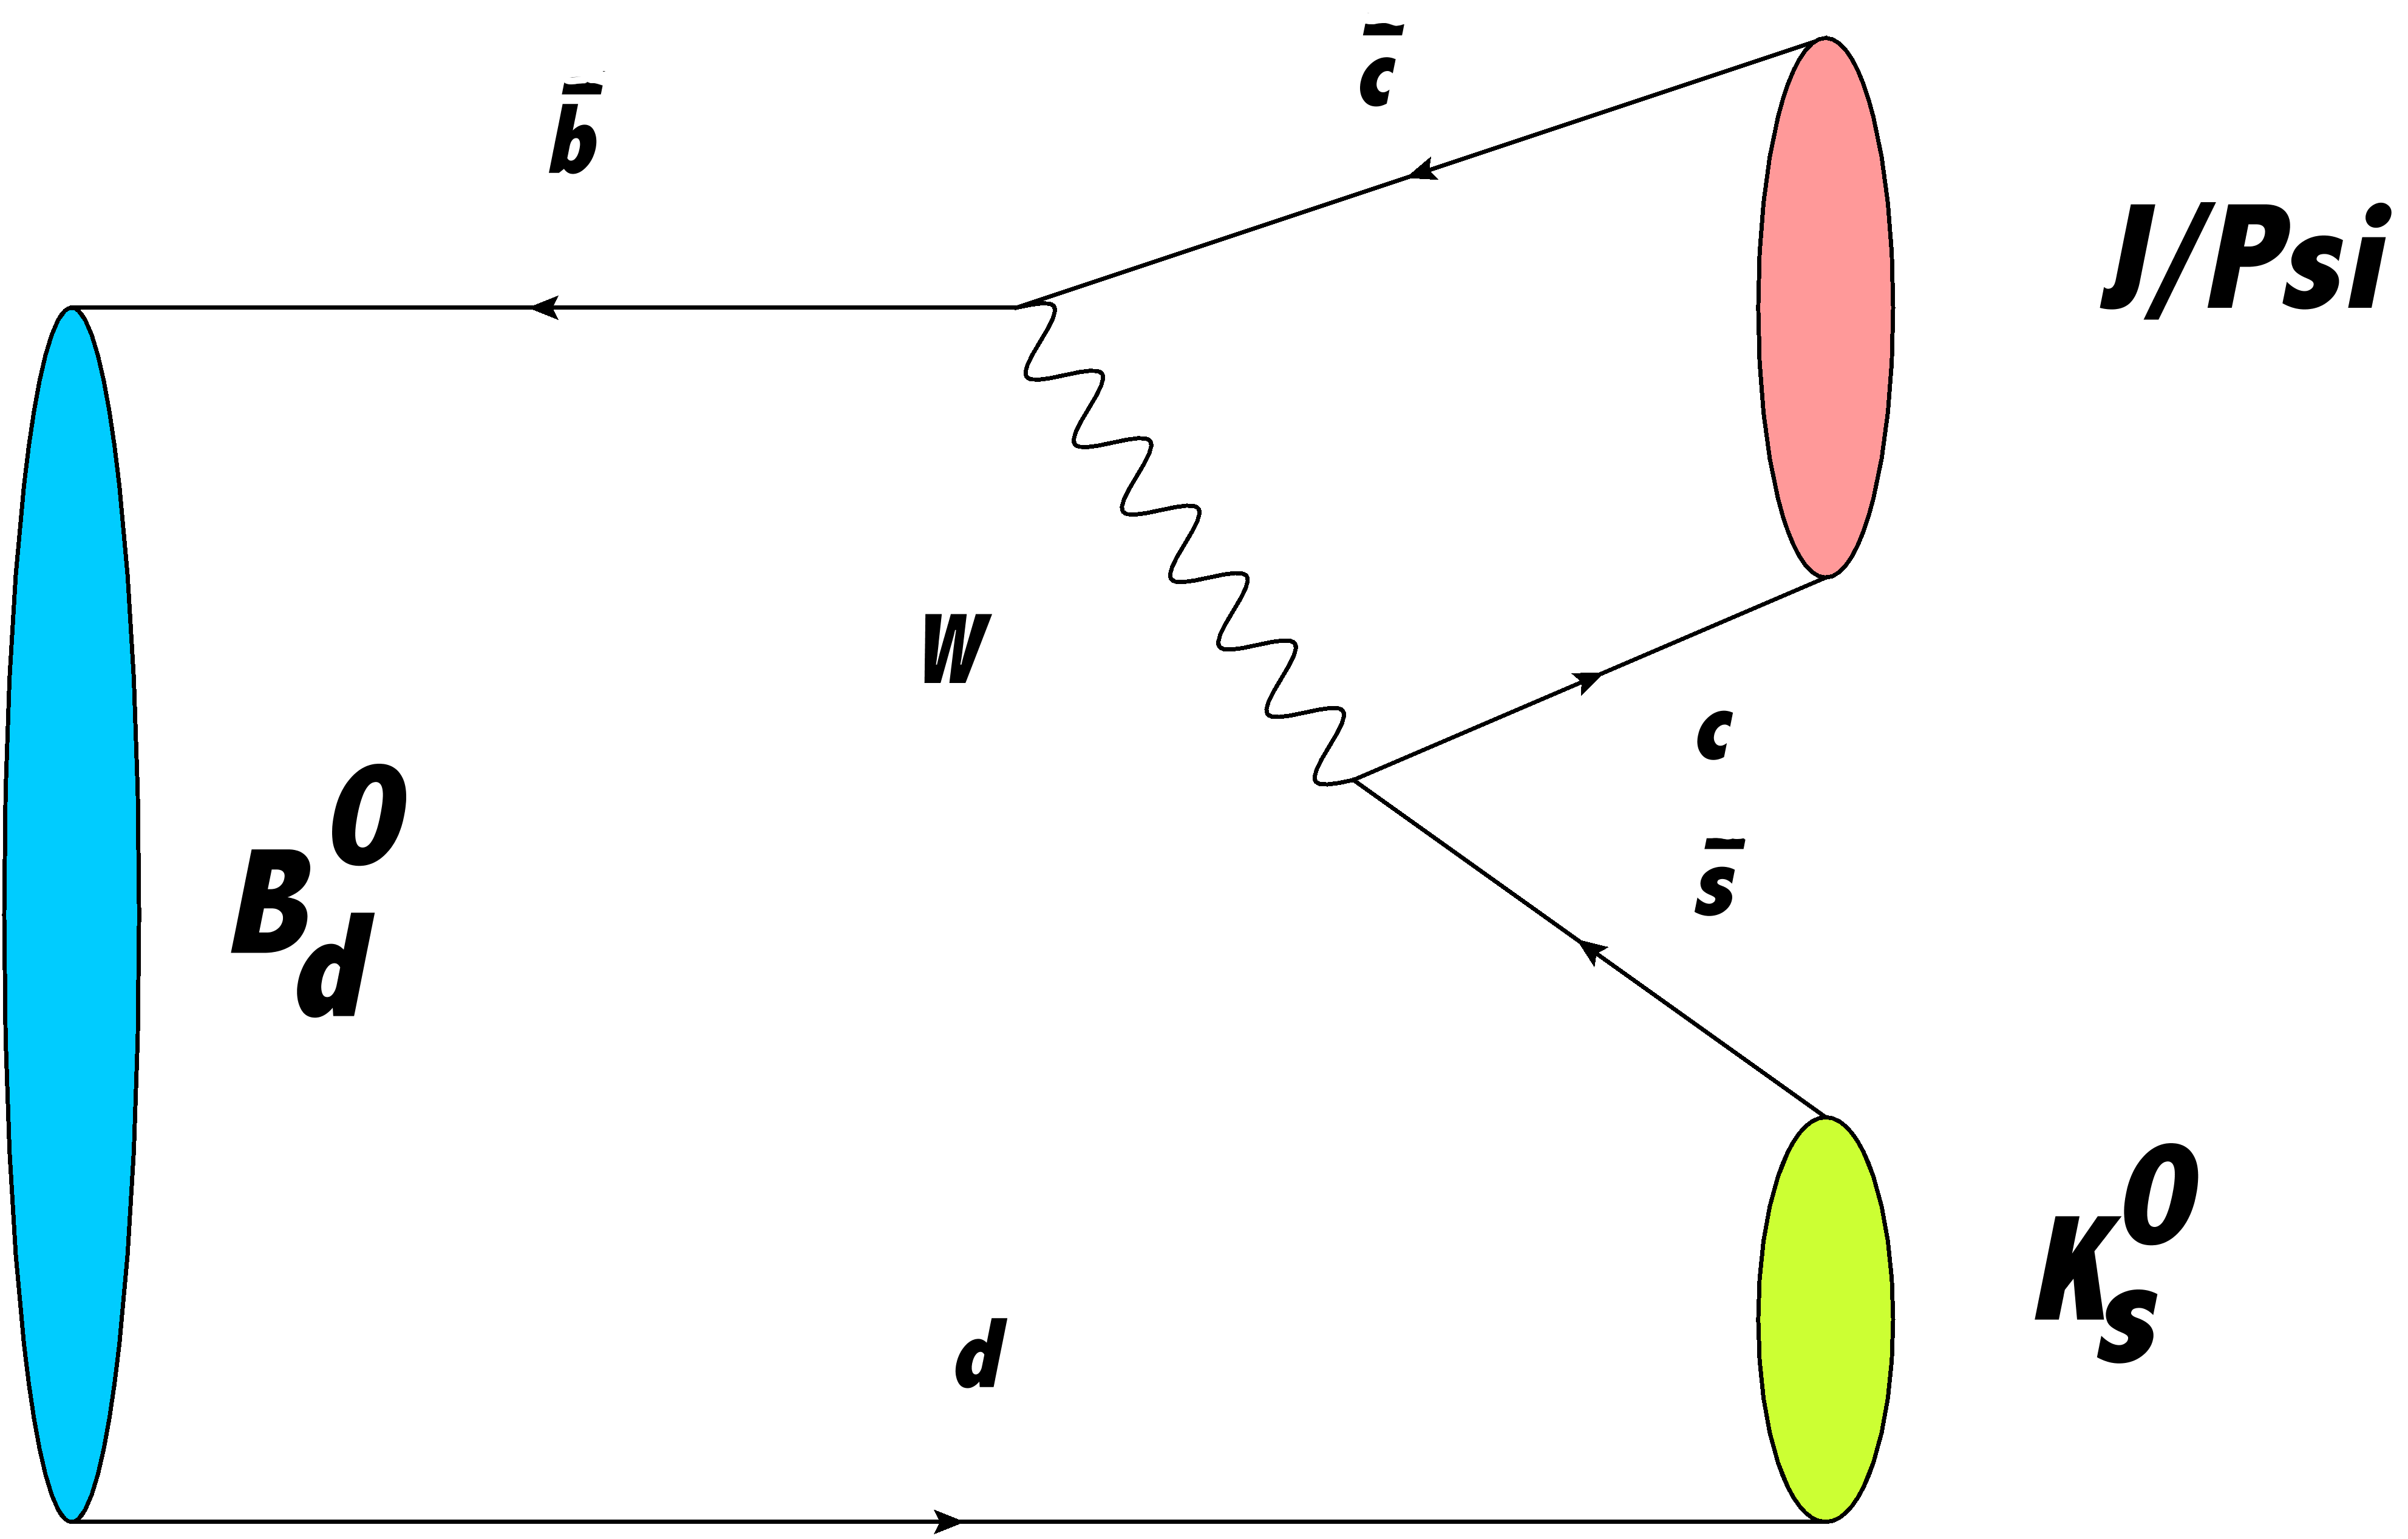
\includegraphics[width=0.5\textwidth]{Decay}
	
\includegraphics[width=0.5\textwidth]{Mixing}
	\begin{center}
	\vspace{1.2cm}
	Measurement of $\mathcal{CP}$-Asymmetry $\mathcal{A_{CP}}$ due to interference between direct decay and decay after mixing
	\end{center}
	\end{frame}

	
	\begin{frame}{Time-dependent asymmetry}
	\begin{align}
	\mathcal{A}_{J/\Psi K_s^0}(t) &= \frac{\Gamma(\bar{B}_d^0 \rightarrow J/\Psi K_s^0)-\Gamma(B_d^0 \rightarrow J/\Psi K_s^0)}{\Gamma(\bar{B}_d^0 \rightarrow J/\Psi K_s^0)+\Gamma(B_d^0 \rightarrow J/\Psi K_s^0)} \\
		&= S_{J/\Psi K_s^0}\sin(\Delta m_d t) - C_{J/\Psi K_s^0}\cos(\Delta m_d t)
	\end{align}
	\begin{columns}
	\column{0.5\textwidth}
	\begin{block}{sine - term}
	\begin{itemize}
		\item interference between direct decay and decay after mixing
		\item $S_{J/\Psi K_s^0} = \sin(2\beta)$
	\end{itemize}
	\end{block}
	
	\column{0.5\textwidth}
	\begin{block}{cosine - term}
	\begin{itemize}
		\item interference between decay amplitudes or CPV in mixing
		\item here: $C_{J/\Psi K_s^0} \approx 0$
	\end{itemize}
	\end{block}
	\end{columns}
	\end{frame}
	
	\begin{frame}{Basis of our work}
	Basis: 2011 LHCb analysis (LHCb-ANA-2012-016)
	\begin{itemize}
	    \item data collected 2011
	    \item $\sqrt{s} = 7\tera\electronvolt$
	    \item $1.025 \mathrm{fb}^{-1}$
	    \item result: $\SJPsi = 0.72 \pm 0.06 \text{(stat.)} \pm 0.04 \text{(syst.)}$
	    \item world average: $\SJPsi = 0.679 \pm 0.020$
	\end{itemize}
	
	Our data:
	\begin{itemize}
	    \item only 2012 data
	    \item $\sqrt{s} = 8\tera\electronvolt$
	    \item $\approx 2 \mathrm{fb}^{-1}$
   	    \item separation into long (Johannes) and downstream (Patrick) tracks
	\end{itemize}
	\end{frame}

	
	\begin{frame}{Cuts}
    \begin{itemize}
    \item in general taken from 2011 analysis
    \item Change in track $\chi^2$ in stripping: $\frac{\chi^2_{\text{track}}}{\text{nDoF}} < 3$ (2011: $<4$)
    \item analysis on stripping line \texttt{BetaSBd2JpsiKsDetachedLine} and HLT2 line \texttt{Hlt2DiMuonDetachedJPsiDecision}
	\item New in 2012: Ghost probability. We choose ghost prob $<0.5$ for $\pi$ and $\mu$ tracks. But issues for Downstream $\pi$ $\rightarrow$ don't use ghost probability of Downstream $\pi$.
	\end{itemize}
	\end{frame}
	
	\begin{frame}{Comparison 2011 $\leftrightarrow$ 2012}
	\begin{center}
	\begin{tabular}{l c c c}
	\hline \hline 
	 & 2011 & long & downstream \\ \hline
	 candidates & 50186 & 21183 & 62184 \\
	 signal & 26775 & 17003 & 42907 \\
	 tagged signal & 8600 & 5116 & 12626 \\ 
	 $\epsilon_{tag}$ & $(32.65 \pm 0.31)\%$ &$(30.09\pm 0.57)\%$ & $(29.43\pm 0.85)\%$ \\
	 $\epsilon_{eff}= \epsilon_{tag}\mathcal{D}^2$ & $(2.38 \pm 0.27)\%$ & $(1.78 \pm xxx)\%$ & $(1.80\pm 0.15)\%$ \\ \hline \hline
	\end{tabular}
	\end{center}
	\vspace{0.5cm}
	Used tagging: FlavourTagging v13r0 2013-06-13 (only OST)
	\end{frame}
	
	\begin{frame}{Fit strategy}
	\begin{itemize}
	\item Unbinned Maximum Likelihood Fit
	\item sFit
	\item total decay time p.d.f.
	\begin{align}
	\mathcal{P}_{meas} = \underbrace{\epsilon(t)}_{= 1,\ \text{later more}}\mathcal{P}_{sig}(t') \otimes \mathcal{R}(t-t')
	\end{align}
	\item neglect decay time acceptance, examination of systematic effect later
	\end{itemize}
	\end{frame}
	
	\begin{frame}{Mean decay time resolution}
	\begin{itemize}
    \item hardly any effect on $\SJPsi$ expected
	\item Resolution model
	\begin{align}
	\mathcal{R}(t) = \sum_{i=1}^3 \frac{f_i}{2\pi\sigma_i}e^{-\tfrac{t^2}{2\sigma^2}}
	\end{align}
	\item Use prescaled trigger line
	\item apply all cuts except lifetime cut
	\item Perform sFit with reonstructed $J/\Psi$ mass as discriminating variable
	\item fit only negative decay times (unphysical, explainable only with resolution effects) ($\rightarrow$ approximation, but sufficient for our purpose)
	\end{itemize}
	\end{frame}
	
	
	\begin{frame}{Mean decay time resolution}
		\begin{columns}
	\column{0.5\textwidth}
	\begin{block}{Long Tracks}
	\centering
	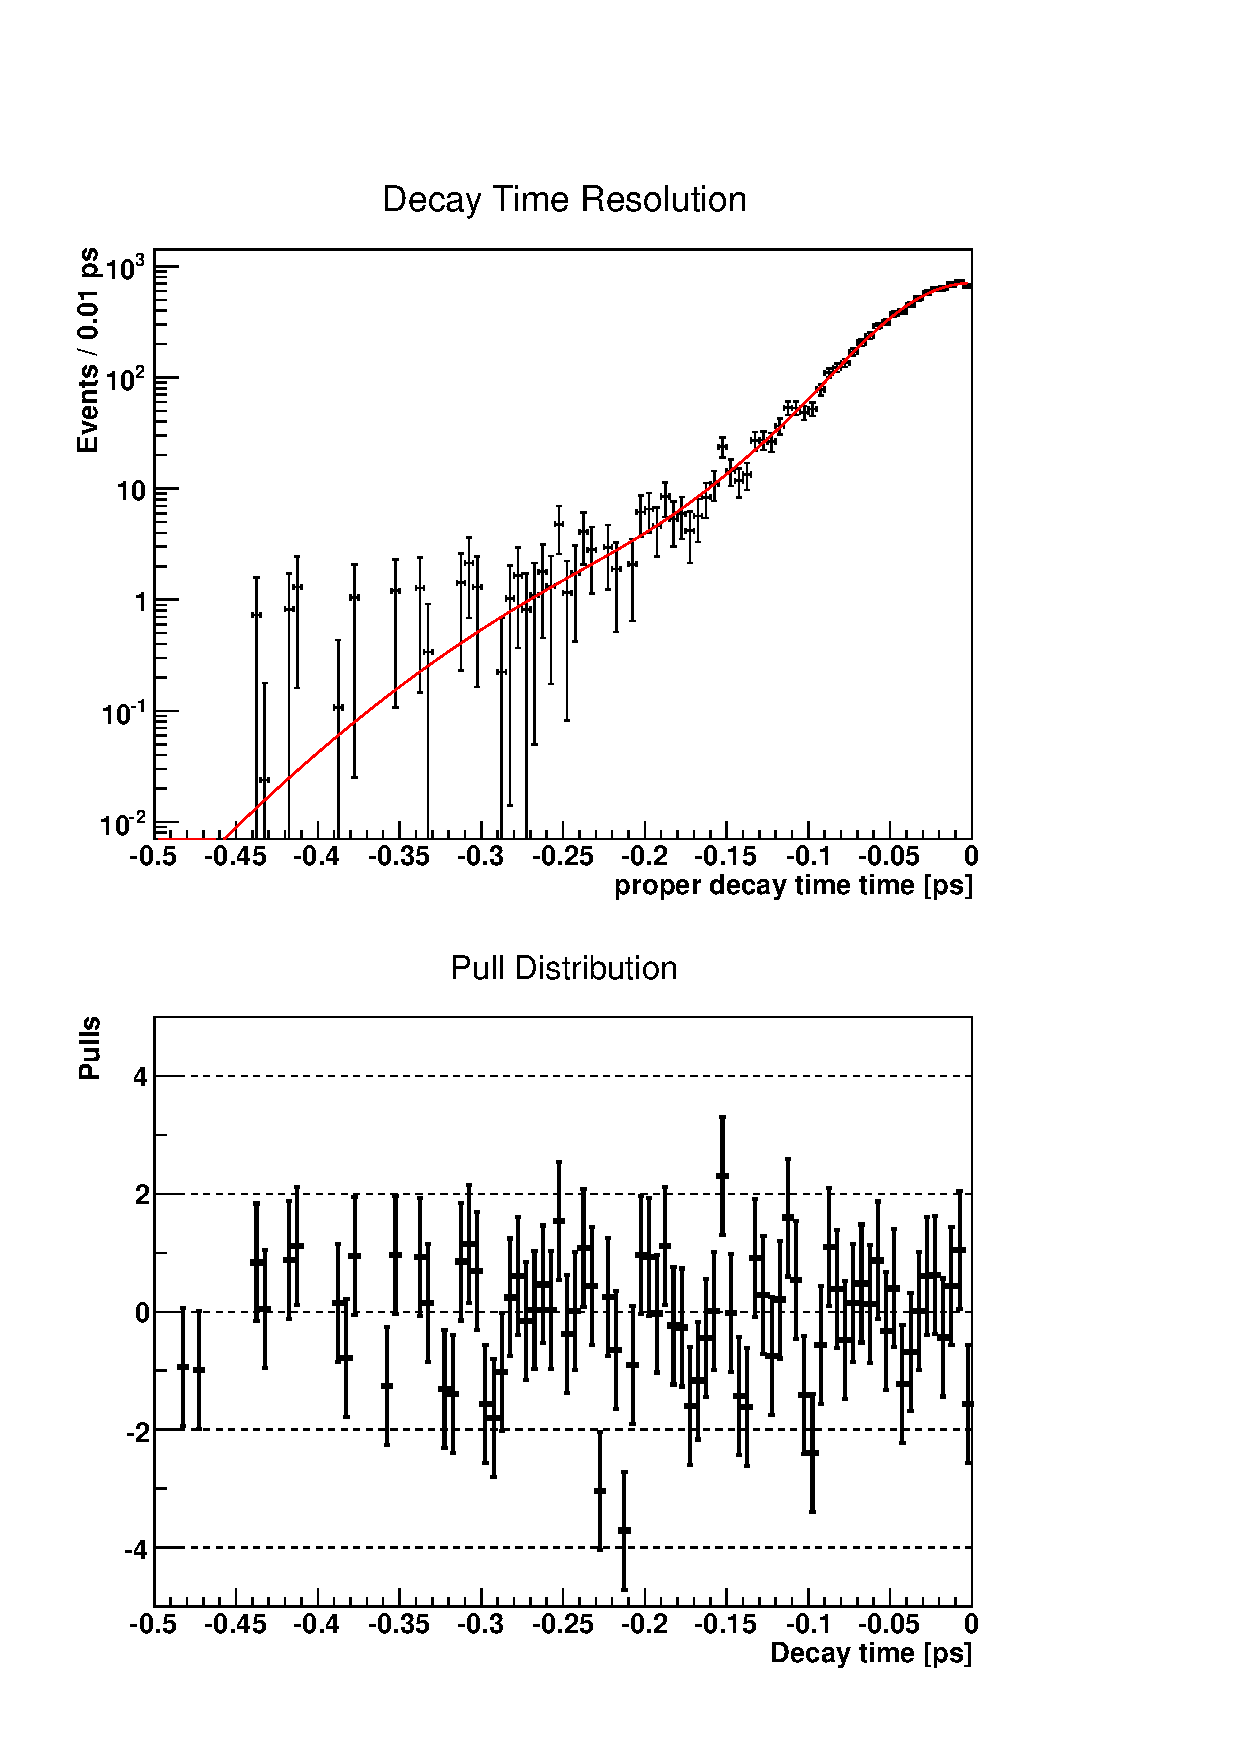
\includegraphics[width=0.92\textwidth]{resolution_lt}
	\end{block}
	\column{0.5\textwidth}
	\begin{block}{Downstream Tracks}
	\centering
	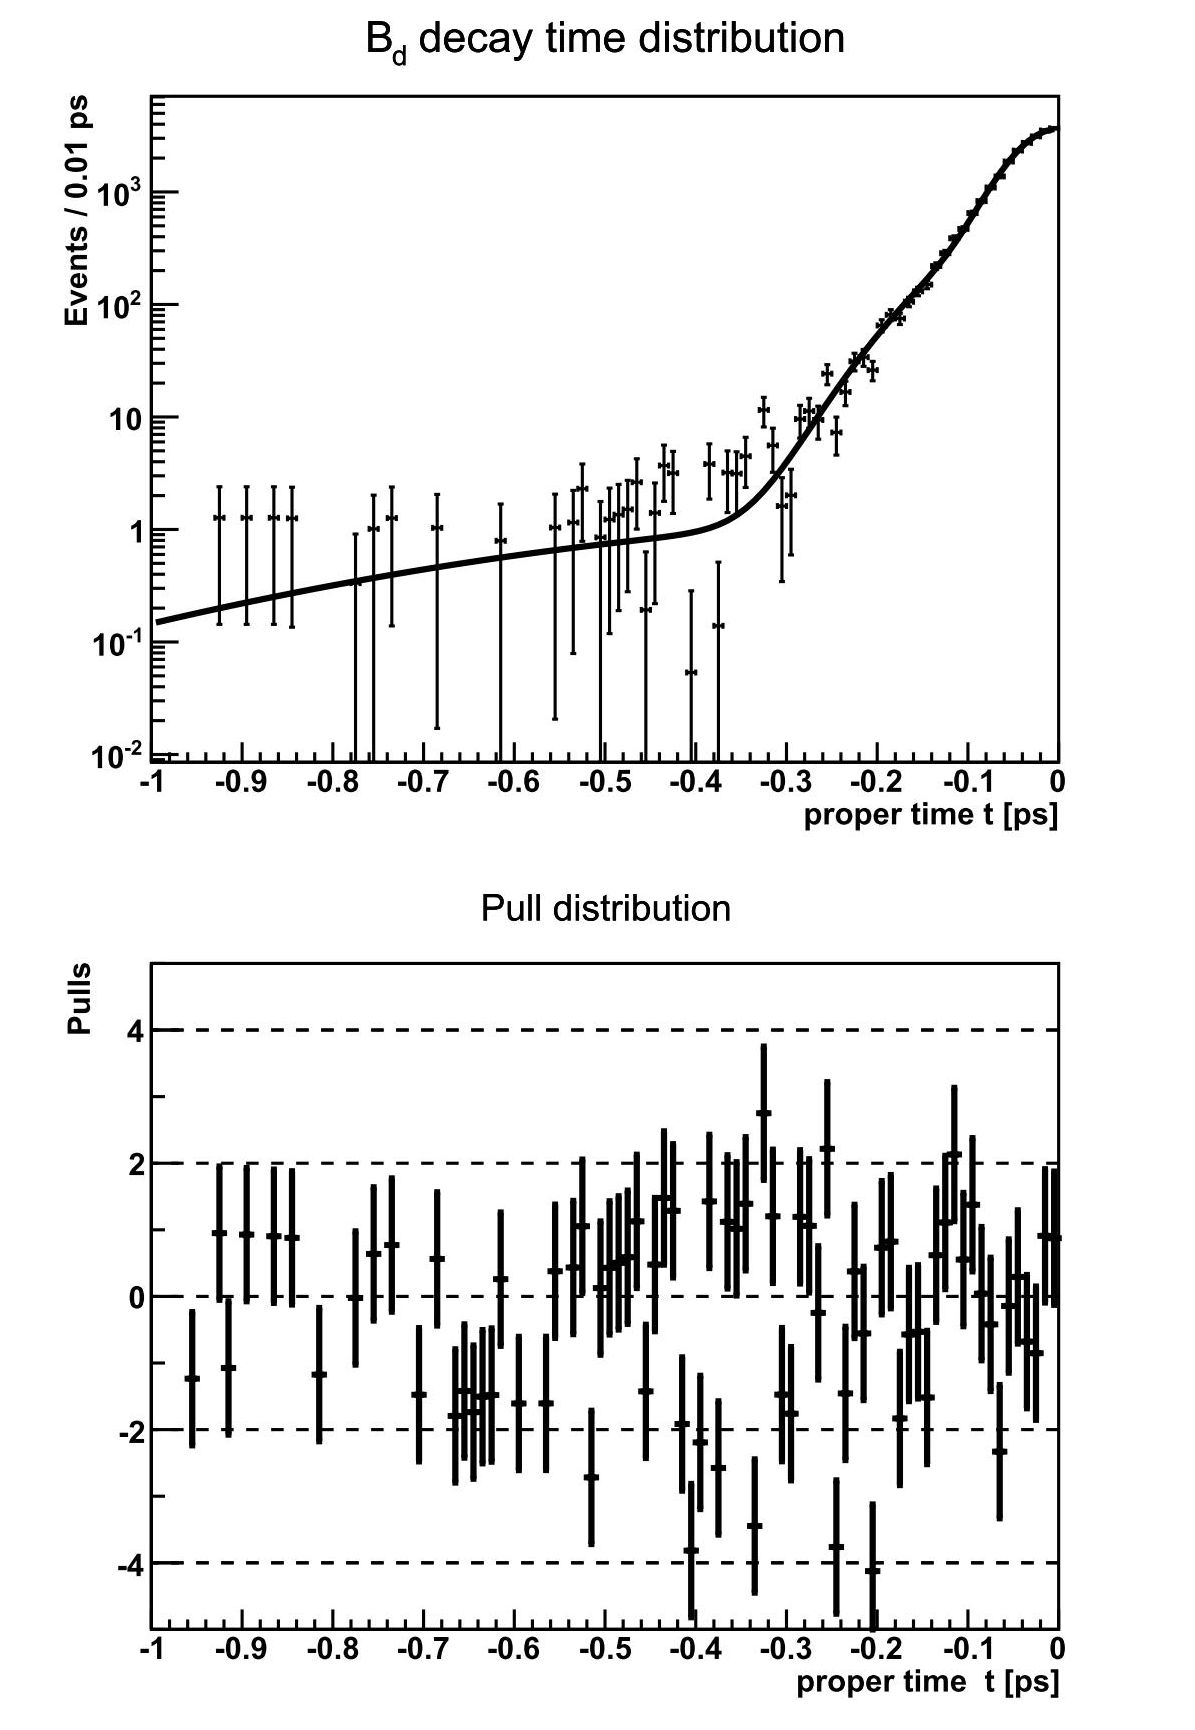
\includegraphics[width=0.95\textwidth]{resolution_ds}
	\end{block}
	\end{columns}
	\end{frame}

    \begin{frame}{Mean decay time resolution}{Fit results}
    \begin{center}
    $\begin{array}{l | r@{\pm}l | r@{\pm}l}
\hline 
\hline
\text{Parameter} & \multicolumn{2}{c|}{\text{long tracks}} & \multicolumn{2}{c}{\text{downstream tracks}}\\
\hline
\sigma_{1}\hspace{1cm}(\text{ps}) &	0.117 & 0.016 & 0.480 & 0.070\\
\sigma_{2}\hspace{1cm}(\text{ps}) &	0.061 & 0.037 & 0.0932 & 0.0034\\
\sigma_{3}\hspace{1cm}(\text{ps}) &0.037 &	0.003 & 0.04396 & 0.00094  \\
f_{1} & 0.054 & 0.032 & 0.00329 & 0.00099\\
f_{2} & 0.294 & 0.138 & 0.257 & 0.027\\ \hline 
\sigma_{eff}\hspace{0.95cm}(\text{ps}) & 0.052 & 0.012 & 0.0665 & 0.0013 \\ \hline \hline
\end{array}$   
    \end{center}
    \end{frame}        	
	
	\begin{frame}{Mass fit}{Parameterisation}
	\begin{block}{Signal}
	\begin{align}
\nonumber \mathcal{P}_{m;S}(m;\vec{\lambda}_{m;S}) = &f_{S,m}\mathcal{G}(m;m_{\text{\Bd}},\sigma_{m,1}) + \\
&(1-f_{S,m})\mathcal{G}(m;m_{\text{\Bd}},\sigma_{m,2})
\end{align}
\end{block}
\begin{block}{Background}
\begin{align}
\mathcal{P}_{m;B}(m;\vec{\lambda}_{m;B}) = e^{-\alpha_m m}/\mathcal{N}_{m;B}
\end{align}
\end{block}
\begin{block}{Total mass p.d.f.}
\begin{align}
\mathcal{P}_{m}(m;\vec{\lambda}_{m}) = f_{sig}\mathcal{P}_{m;S}(m;\vec{\lambda}_{m;S}) + (1-f_{sig})\mathcal{P}_{m;B}(m;\vec{\lambda}_{m;B})
\end{align}
\end{block}
	\end{frame}
	
	\begin{frame}{Mass fit}
	\begin{columns}
	\column{0.5\textwidth}
	\begin{block}{Long Tracks}
	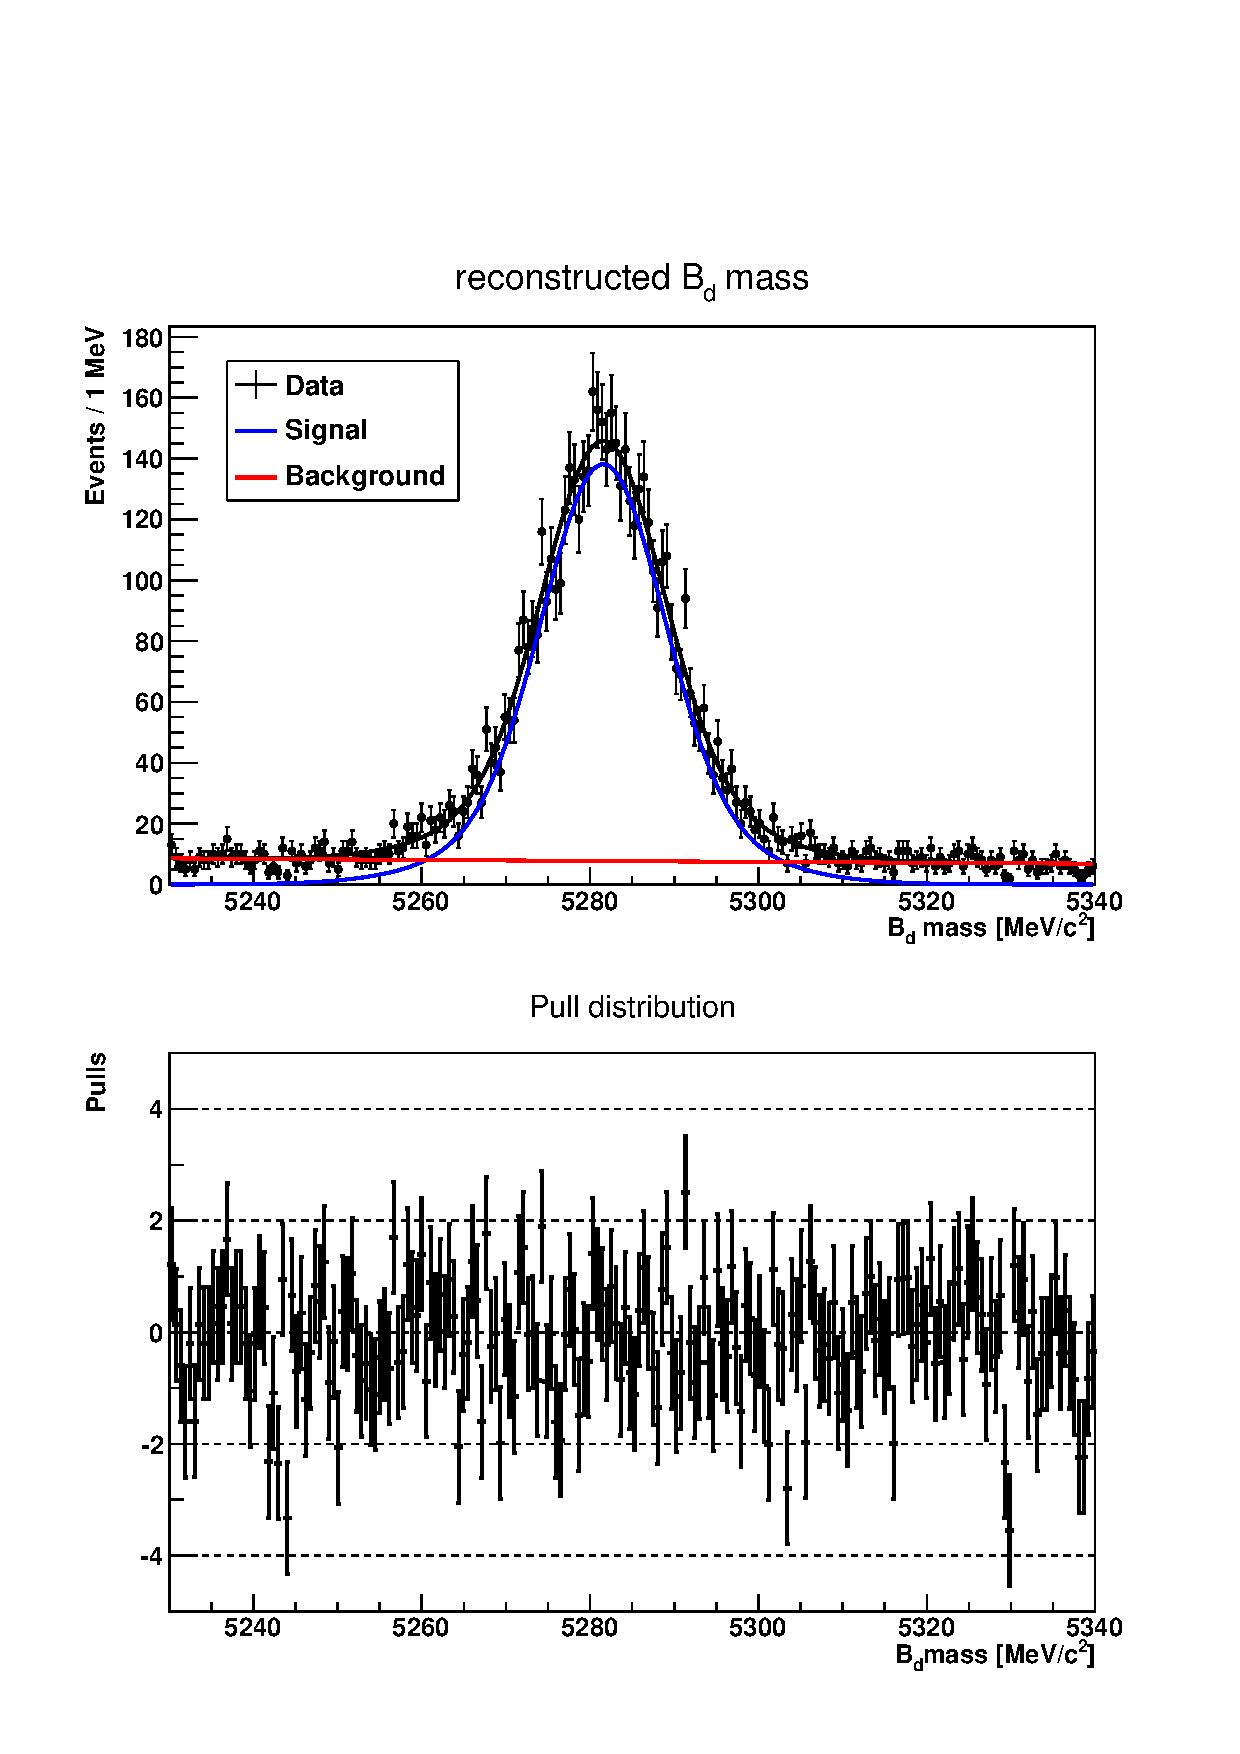
\includegraphics[width=\textwidth]{mass_fit_lt}
	\end{block}
	\column{0.5\textwidth}
	\begin{block}{Downstream Tracks}
	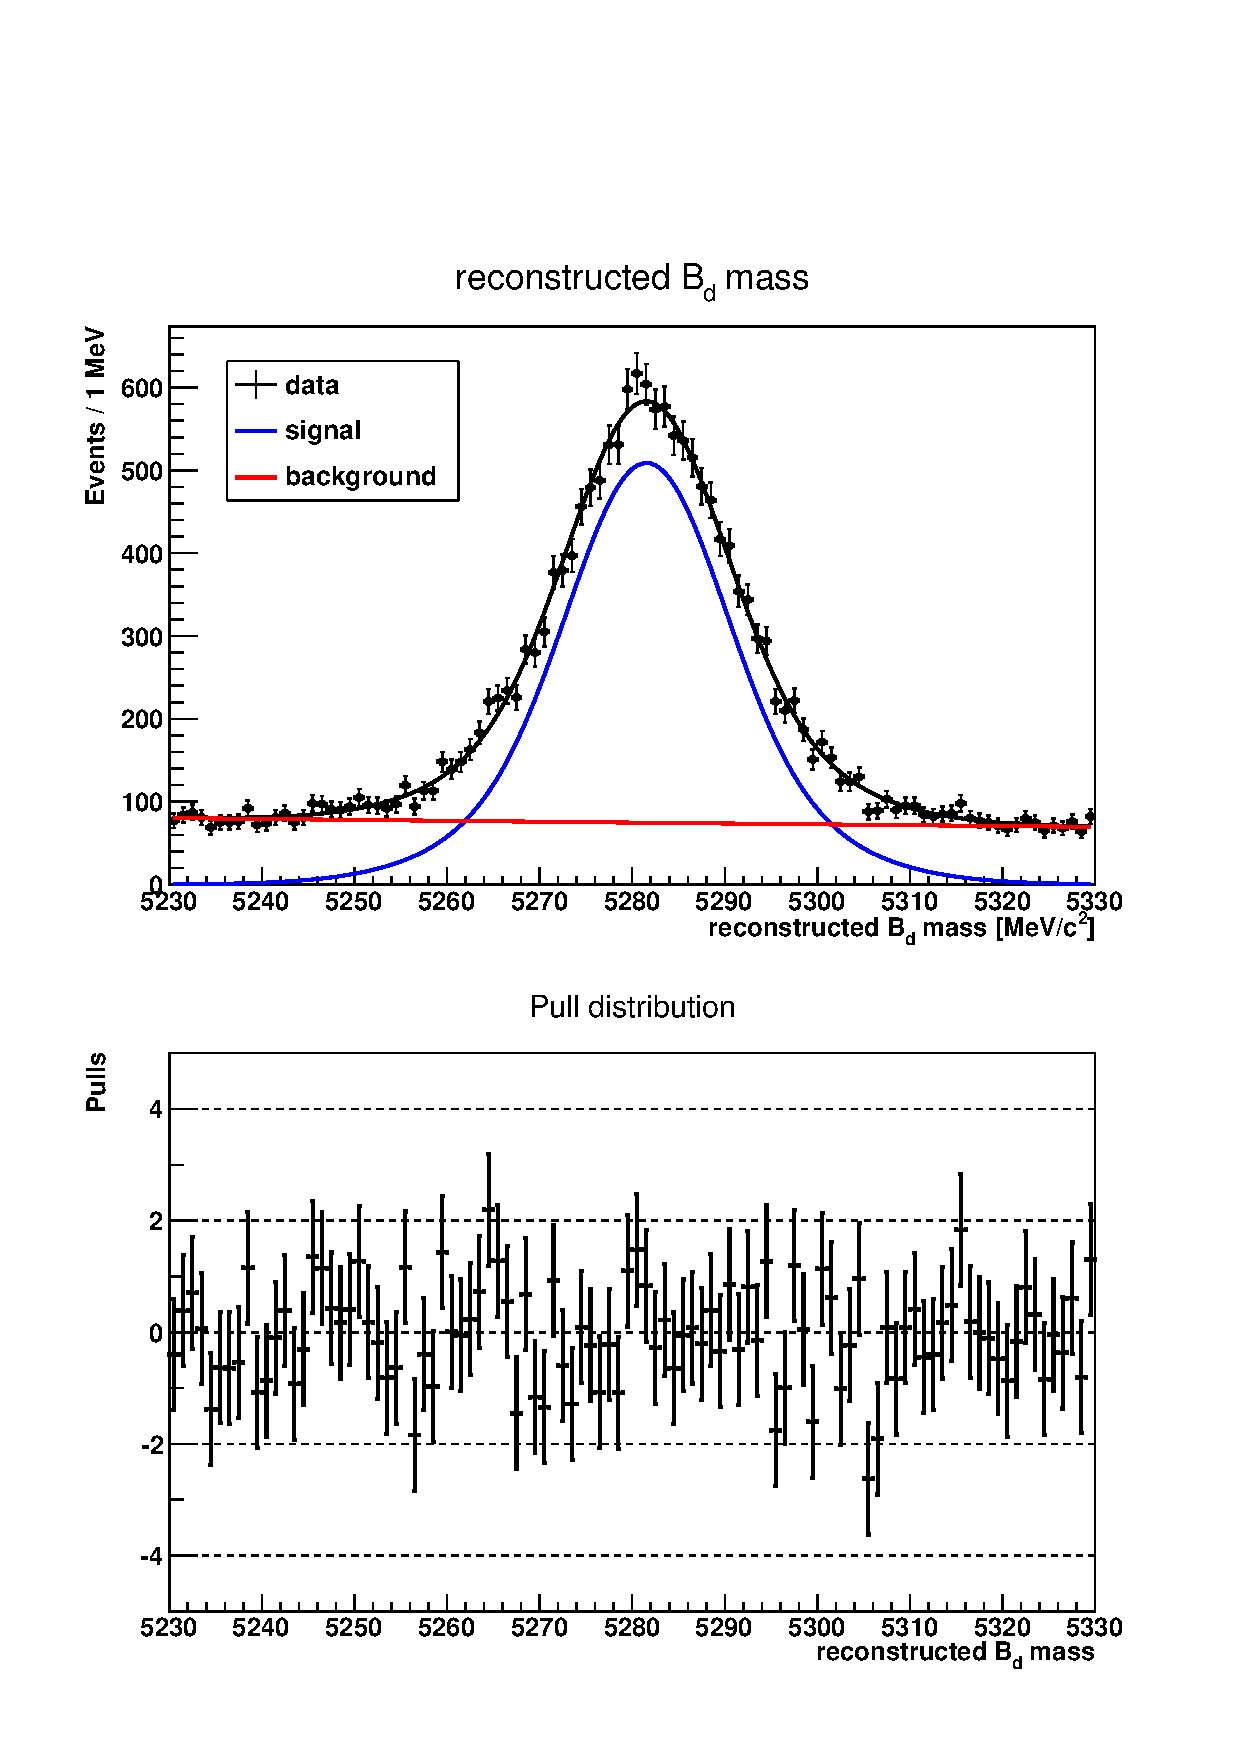
\includegraphics[width=\textwidth]{mass_fit_ds}
	\end{block}
	\end{columns}
	\end{frame}
	
	
	\begin{frame}{Decay time fit}{probability density function used in fit}
	\begin{align}
\nonumber\mathcal{P}_{\text{meas}}(t, d, \omega) \propto &e^{-t/\tau} \left\lbrace 1-d\mu(1-2\omega)-d\Delta p_0 \right. \\
&- \left.\left[d(1-2\omega)-\mu(1-d\Delta p_0)\right]\SJPsi\sin(\Delta m_d t)\right\rbrace
	\end{align}	
	\begin{itemize}
		\item d: tagging decision
		\item $\mu = A_P = \frac{R_{\bar{B}_d^0}-R_{B_d^0}}{R_{\bar{B}_d^0}+R_{B_d^0}}$ production asymmetry
		\item $\omega$: calibrated mistag probability
		      \begin{align}
		      \omega(\eta^{OS}) = p_1 (\eta^{OS} - \left\langle \eta^{OS} \right\rangle) + p_0
		      \end{align}
		      $p_0, p_1$: calibration parameters \\
		      $\eta^{OS}$: predicted mistag probability
		\item $\Delta p_0$: tagging calibration asymmetry
		\item $\Delta m_d$: mixing frequency

	\end{itemize}	
	\end{frame}
	
	
	\begin{frame}{Fit results}
	\begin{itemize}
		\item floating parameters: $S_{J/\Psi K_s^0}$, $\tau$, $\Delta m_d$
		\item constrained parameters: $\mu = -0.015\pm0.013$, $p_0 = 0.382\pm0.003$, $p_1=0.981\pm0.024$, $\Delta p_0 = 0.0045\pm0.0053$
		\item fixed parameters: $\left\langle \eta^{OS} \right\rangle = 0.382$, resolution parameters
	\end{itemize}
	\end{frame}

	
	\begin{frame}{Fit results}
	\begin{columns}
	\column{0.5\textwidth}
	\begin{block}{Long Tracks}
	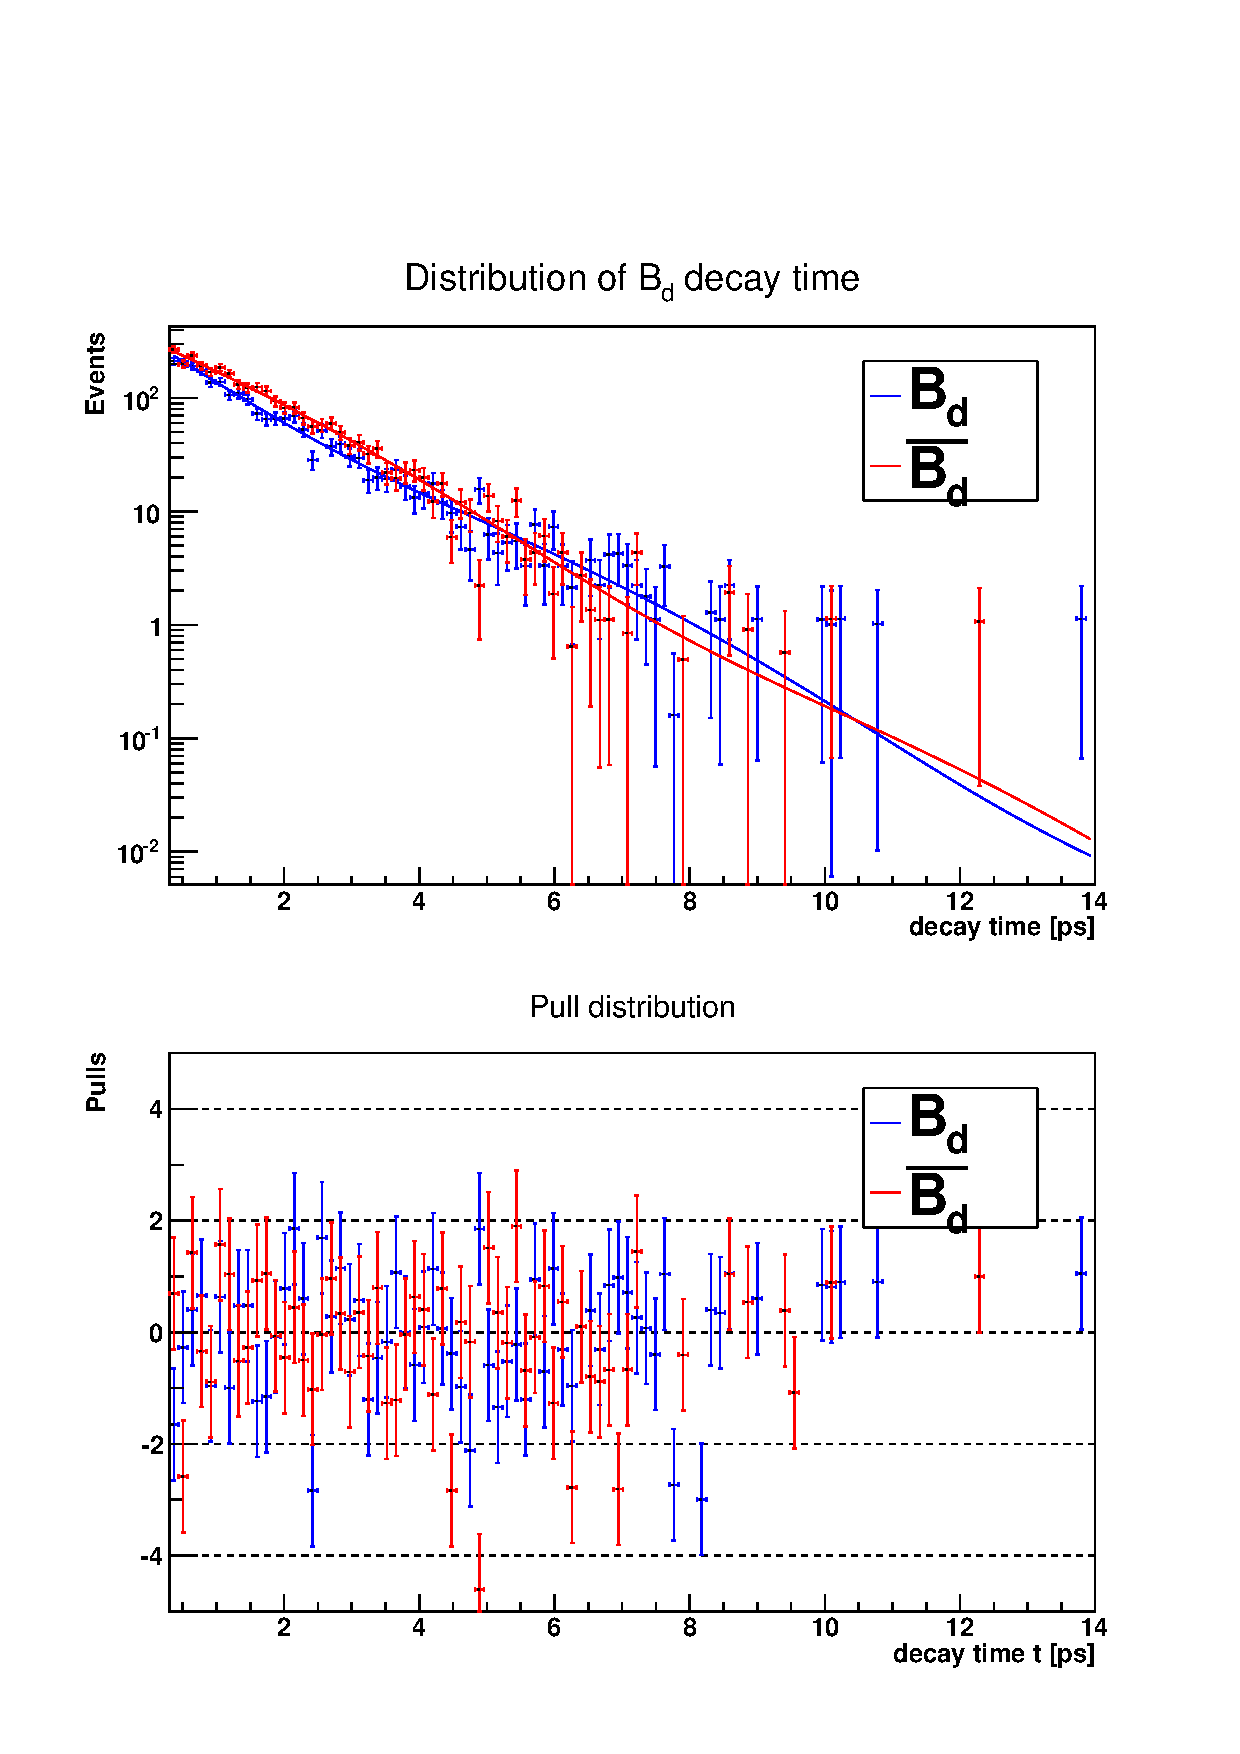
\includegraphics[width=\textwidth]{decay_distribution_lt}
	\end{block}
	\column{0.5\textwidth}
	\begin{block}{Downstream Tracks}
	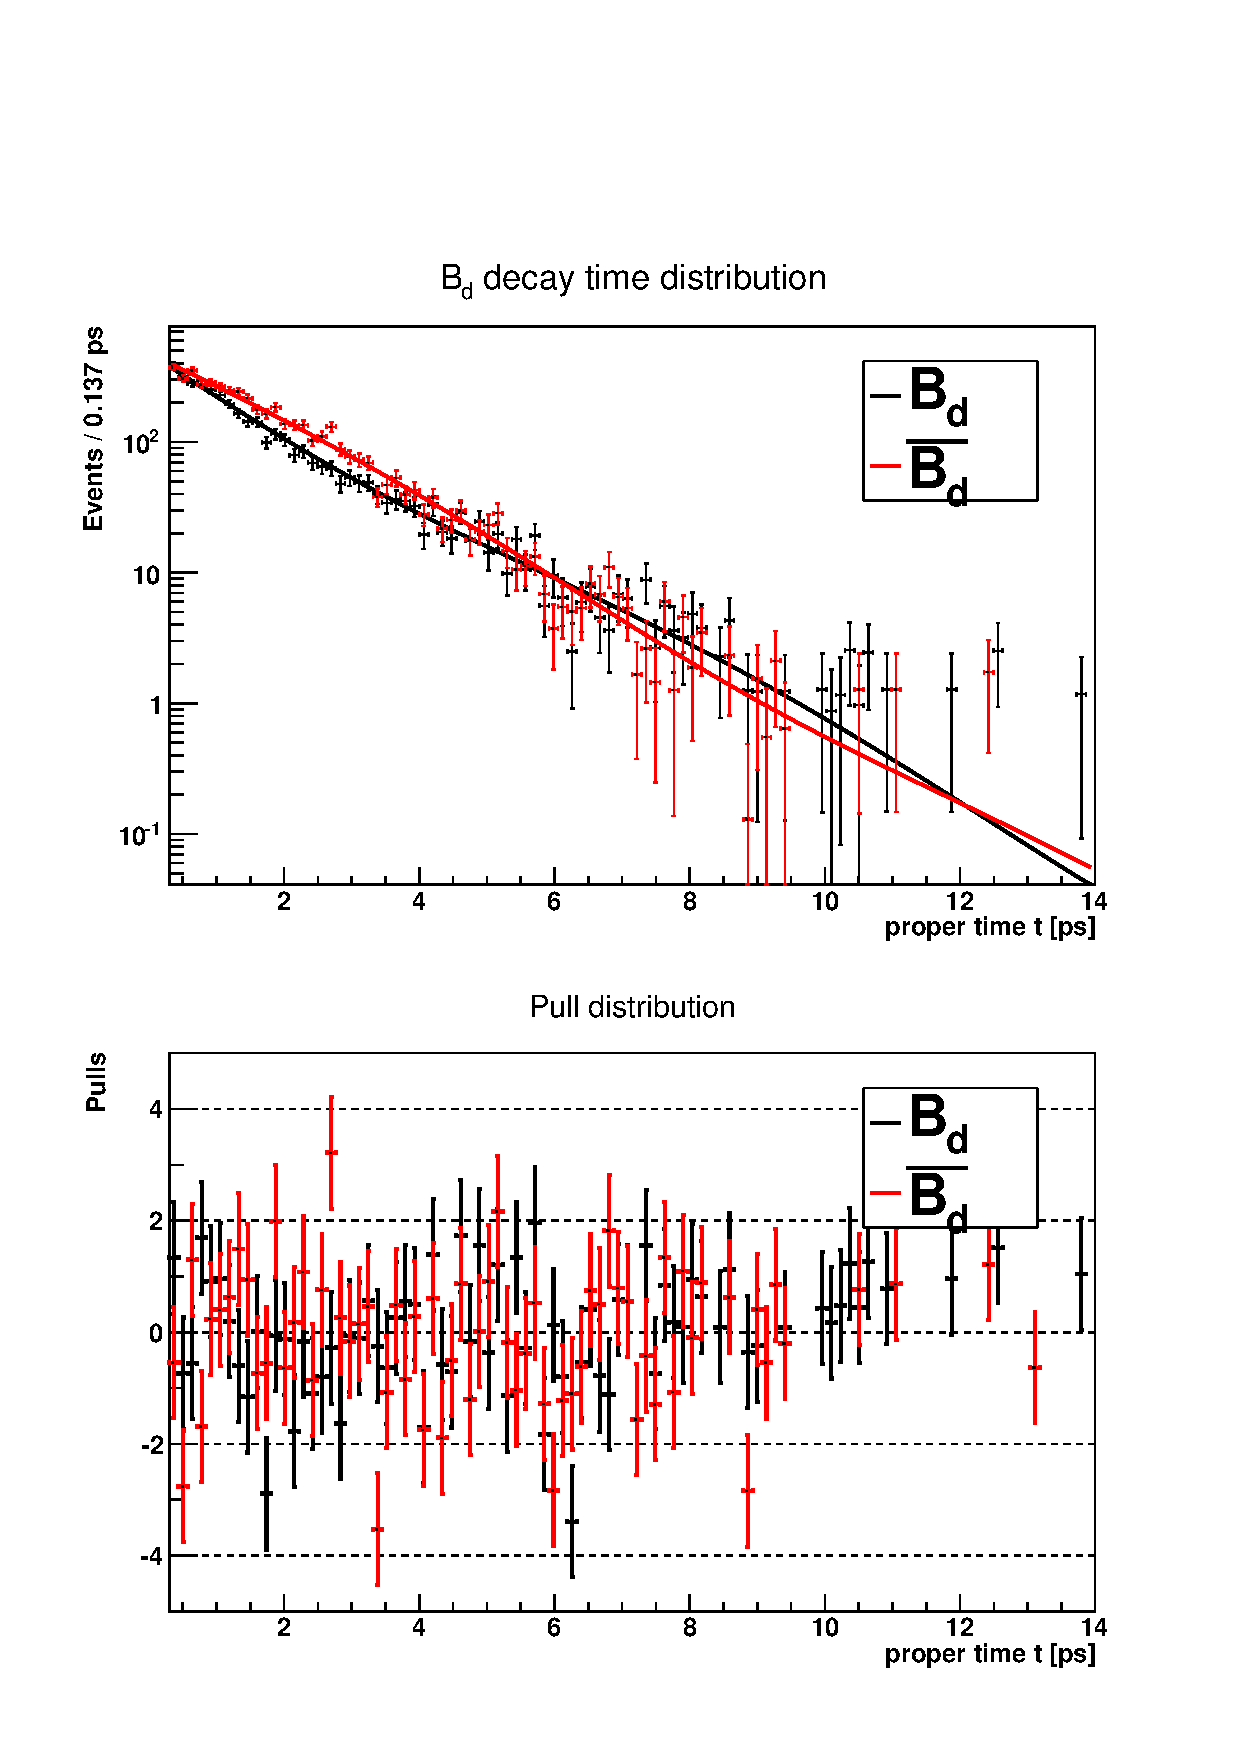
\includegraphics[width=\textwidth]{decay_distribution_ds}
	\end{block}
	\end{columns}

	\end{frame}
	
	\begin{frame}{Fit results}
	\begin{alert}{Note:}
	Both results of $\SJPsi$ are blinded with the same string.
	\end{alert}
	\begin{center}
	$\begin{array}{l r@{\pm}l r@{\pm}l}
	\hline \hline
	\text{Parameter} & \multicolumn{2}{c}{\text{long}} & \multicolumn{2}{c}{\text{downstream}}\\ \hline
	\SJPsi (\text{blinded}) & 0.610 & 0.078 & 0.535 & 0.063 \\
	\SJPsi (2011)           & xxx   & 0.11  & xxx   & 0.08  \\ \hline
	\tau_{\text{eff}}       & 1.355 & 0.021 & 1.498 & 0.017 \\ \hline
	\Delta m_d         & 0.60 & 0.05 & 0.47 & 0.03 \\
    \Delta m_d (2011)  & 0.58 & 0.15 & 0.50 & 0.04 \\
	\hline
	\end{array}$
	\end{center}
    \begin{alert}{Note:}
	$\tau_{eff}$ not compatible to PDG value due to neglect of time acceptance in fit (systematic study later)
	\end{alert} \\
	\begin{alert}{Question:}
	Why is $\Delta m_d$ that much higher in the long track sample?
	\end{alert}
	\end{frame}

	
	\begin{frame}{Systematic errors}
	\begin{itemize}
		\item Fit Bias due to fit method sFit
	    \item Tagging calibration
	    \item Time acceptance
	    \item Correlation mass $\leftrightarrow$ decay time
	    \item Time resolution
	\end{itemize}
	\end{frame}
	
	\begin{frame}{Systematic errors}{Fit Bias}
	Generate Toy MC with 
	\begin{itemize}
	\item 6700 (long) resp. 20000 events (downstream)
	\item $\SJPsi = 0.72$ 
	\item all other parameters derived from data fit
	\item $\SJPsi$, $\tau$, $\Delta m_d$ floating
	\end{itemize}
    \end{frame}	
	
	\begin{frame}{Systematic errors}{Fit Bias}
	\begin{columns}
	\column{0.5\textwidth}
	\begin{block}{Long Tracks}
	\centering
	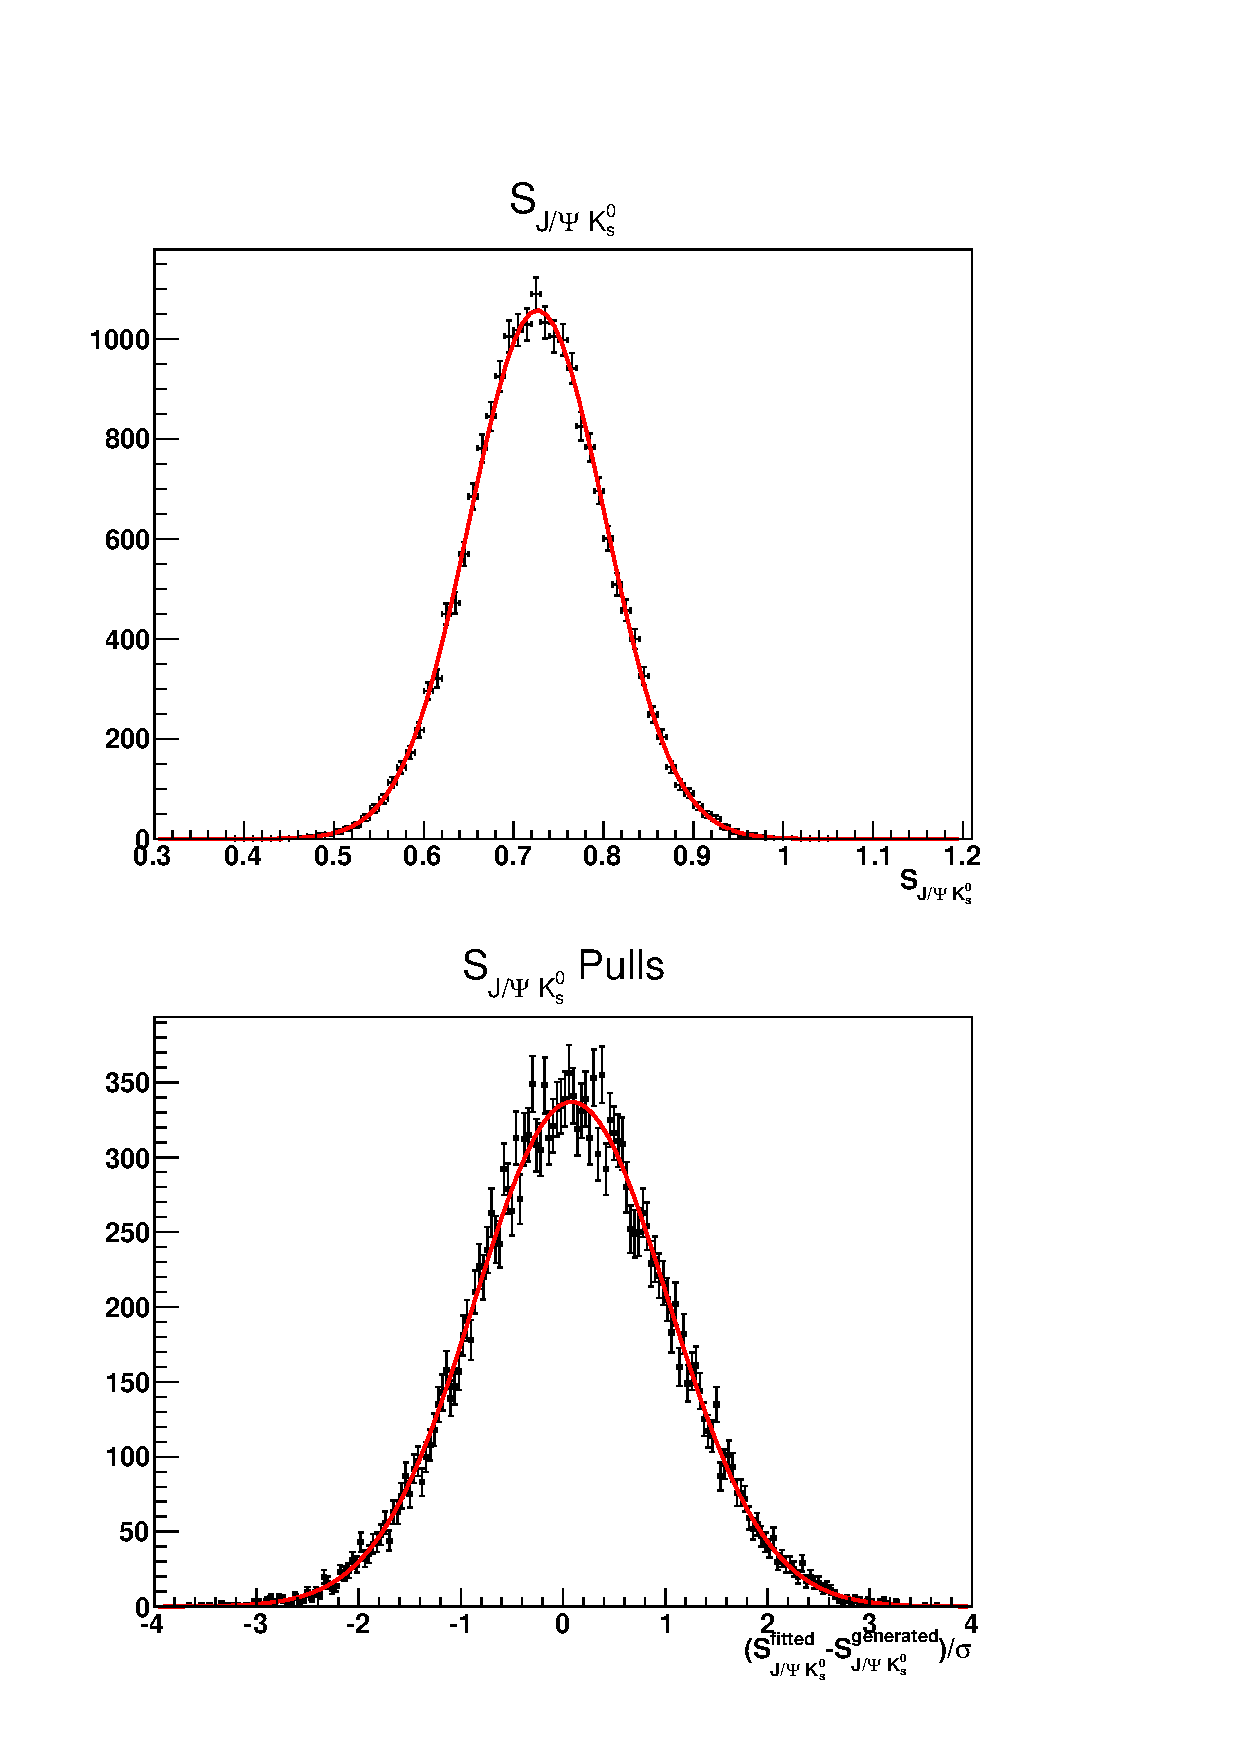
\includegraphics[width=\textwidth]{fit_bias_lt}	
	\end{block}
	\column{0.5\textwidth}
	\begin{block}{Downstream Tracks}
	\centering
	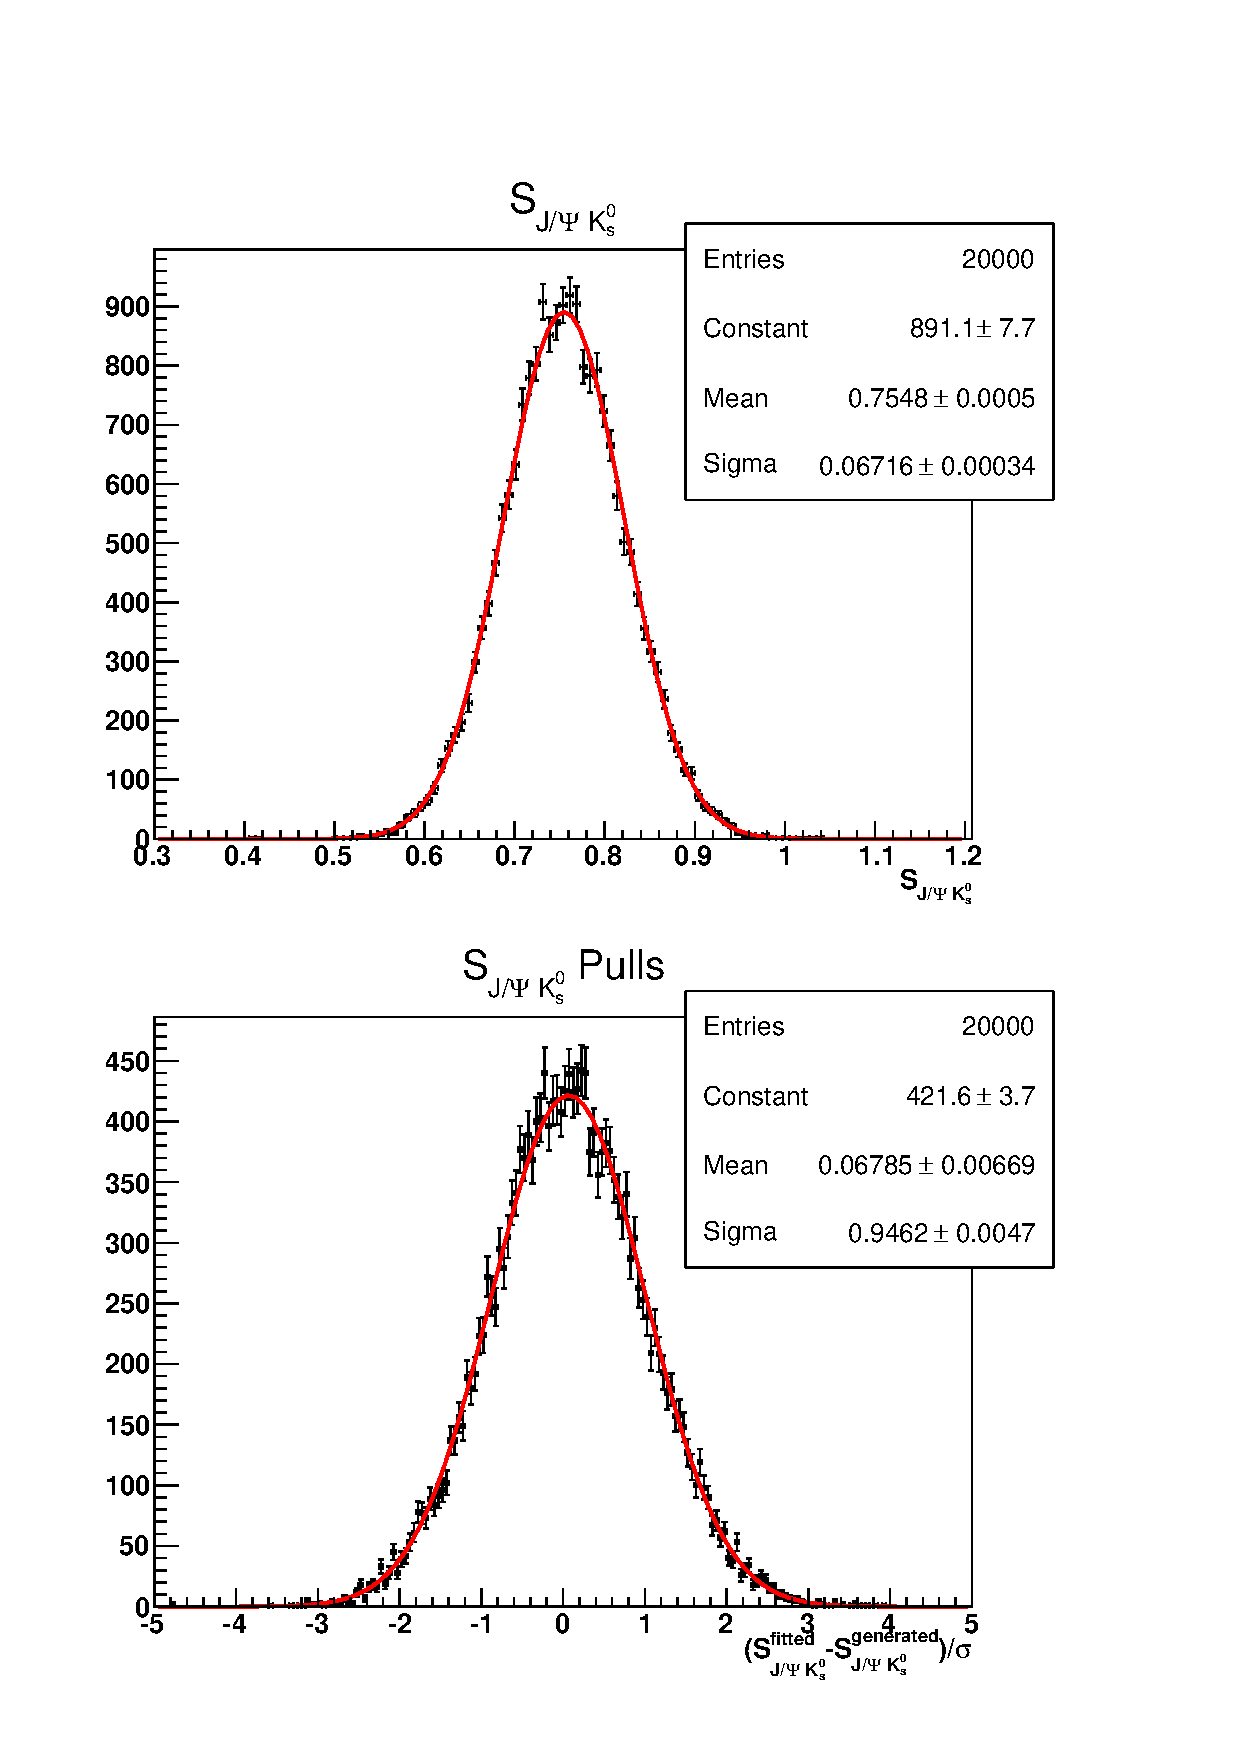
\includegraphics[width=0.8\textwidth]{fit_bias_ds}
	\end{block}
	\end{columns}
	\end{frame}
	
	\begin{frame}{Systematic errors}{Fit Bias}
	Results of the toys:
	\begin{columns}
	\column{0.5\textwidth}
	\begin{block}{Long Tracks}
        $\mu_{\SJPsi} = 0.7266 \pm 0.0005$
        $\sigma_{\SJPsi} = 0.0754 \pm 0.0003$
        $\mu_{\text{pull}} = 0.083 \pm 0.007$
        $\sigma_{\text{pull}} = 0.947 \pm 0.005$
    \end{block}
    	\column{0.5\textwidth}
	\begin{block}{Downstream Tracks}
    
        $\mu_{\SJPsi} = 0.7234 \pm 0.0004$
        $\sigma_{\SJPsi} = 0.0584 \pm 0.0003$
        $\mu_{\text{pull}} = 0.052 \pm 0.007$
        $\sigma_{\text{pull}} = 0.941 \pm 0.005$
    \end{block}
    \end{columns}
	\vspace{0.5cm} 
	Multiply mean $\mu_{\text{pull}}$ of pull distribution with statistical uncertainty of nominal fit (long: $\sigma_{\text{data}}=0.078$, down: $\sigma_{\text{data}}=0.063$).
	\begin{columns}
	\column{0.5\textwidth}
	\begin{block}{Long Tracks}
    \centering
        $\delta\SJPsi^{\text{Fit}} = 0.0066\ (8.5\%)$
    \end{block}
    	\column{0.5\textwidth}
	\begin{block}{Downstream Tracks}
    \centering
        $\delta\SJPsi^{\text{Fit}} = 0.0033\ (5.2\%)$
    \end{block}
    \end{columns}
    \vspace{0.5cm}
    (in Brackets: systematic error relative to systematic)
    \end{frame}
	
	\begin{frame}{Systematic errors}{Fit Bias - origins}
    \begin{itemize}
      \item major contribution to bias: too little statistics
      \begin{center}
    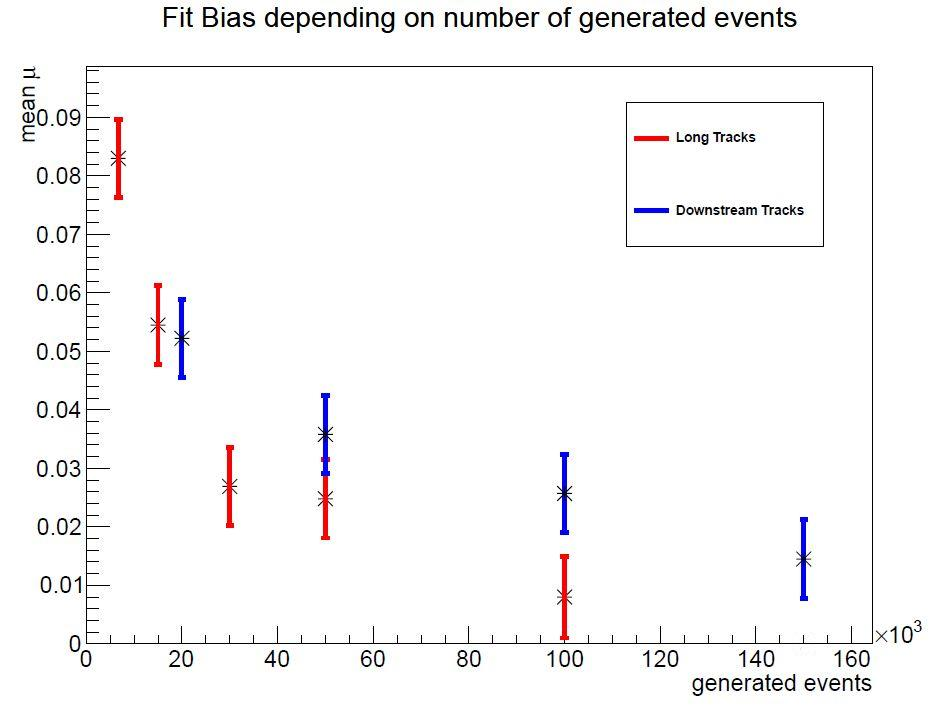
\includegraphics[width = 0.6\textwidth]{fit_bias_statistics}
    \end{center}
    \item too small pull width due to background ($\rightarrow$ overestimation of fit error)
    \item $\sigma_{\text{pull}}$ doesn't change with higher statistics
    \end{itemize}
    
    \end{frame}
	
	\begin{frame}{Systematic errors}{Tagging calibration}
	Vary Tagging calibration parameters $p_0, p_1$ $\pm$ their systematic uncertainties
	\begin{enumerate}
	\item in the nominal fit (gives first impression of size of effect)
	\item in the generation of Toy MC, but fit with original values
	\end{enumerate}
	\begin{alert}{Note:}
	Systematic studies on used tagging calibration hasn't finished yet $\longrightarrow$ no official value. Use systematic errors of 2011 (to get a feeling for size of effect, need to be redone with final calibration):
	\begin{align*}
	\delta p_0^{stat.} = 0.0076, \qquad \delta p_1^{stat.} = 0.0012
	\end{align*}
	\end{alert}
	Choose highest difference from nominal fit bias toy as estimate for the systematic uncertainty
	\begin{itemize}
	\item Long tracks: $\delta\SJPsi^{\text{TagCalib}} = 0.0320\ (41.0\%)$
	\item Downstream tracks: $\delta\SJPsi^{\text{TagCalib}} = 0.0331\ (52.5\%)$
    \end{itemize}		    
    \end{frame}
    
    \begin{frame}{Systematic errors}{Time acceptance}
    \begin{alert}{Note:}
    just a cross-check, no in-depth analysis
    \end{alert}
    \begin{block}{Determination of an acceptance function}
    \begin{itemize}
    \item no separation between \Bd \ and \Bdbar \\
          $\Rightarrow$ simple exponential decay
    \item neglect lifetime cut ($t > 0.3\text{ps}$)
    \item contributions to acceptance:
          \begin{itemize}
          \item turn-on-effect
          \item decreasing acceptance for higher lifetimes due to VELO geometry
          \end{itemize}
    \end{itemize}
    \end{block}
\end{frame}

\begin{frame}{Systematic errors}{Time acceptance}
    \begin{block}{Fit p.d.f}
    $\mathcal{P}_{acc}(t) \propto \underbrace{e^{-t/\tau}}_{\text{exp. decay}} \cdot \underbrace{\frac{2}{\pi}\arctan[t\cdot \exp(at+b)]}_{\text{turn-on-effect}} \cdot \underbrace{(1 + \beta t)}_{\substack{\text{higher lifetimes} \\(\beta<0)}}$
    \end{block}
    \begin{alert}{Note:}
    $\tau$ will be constrained to the PDG value $\tau = 1.519 \pm 0.007 \pico\second$.
    \end{alert}
\end{frame}

\begin{frame}{Systematic errors}{Time acceptance}
\begin{block}{Long Tracks}
\centering
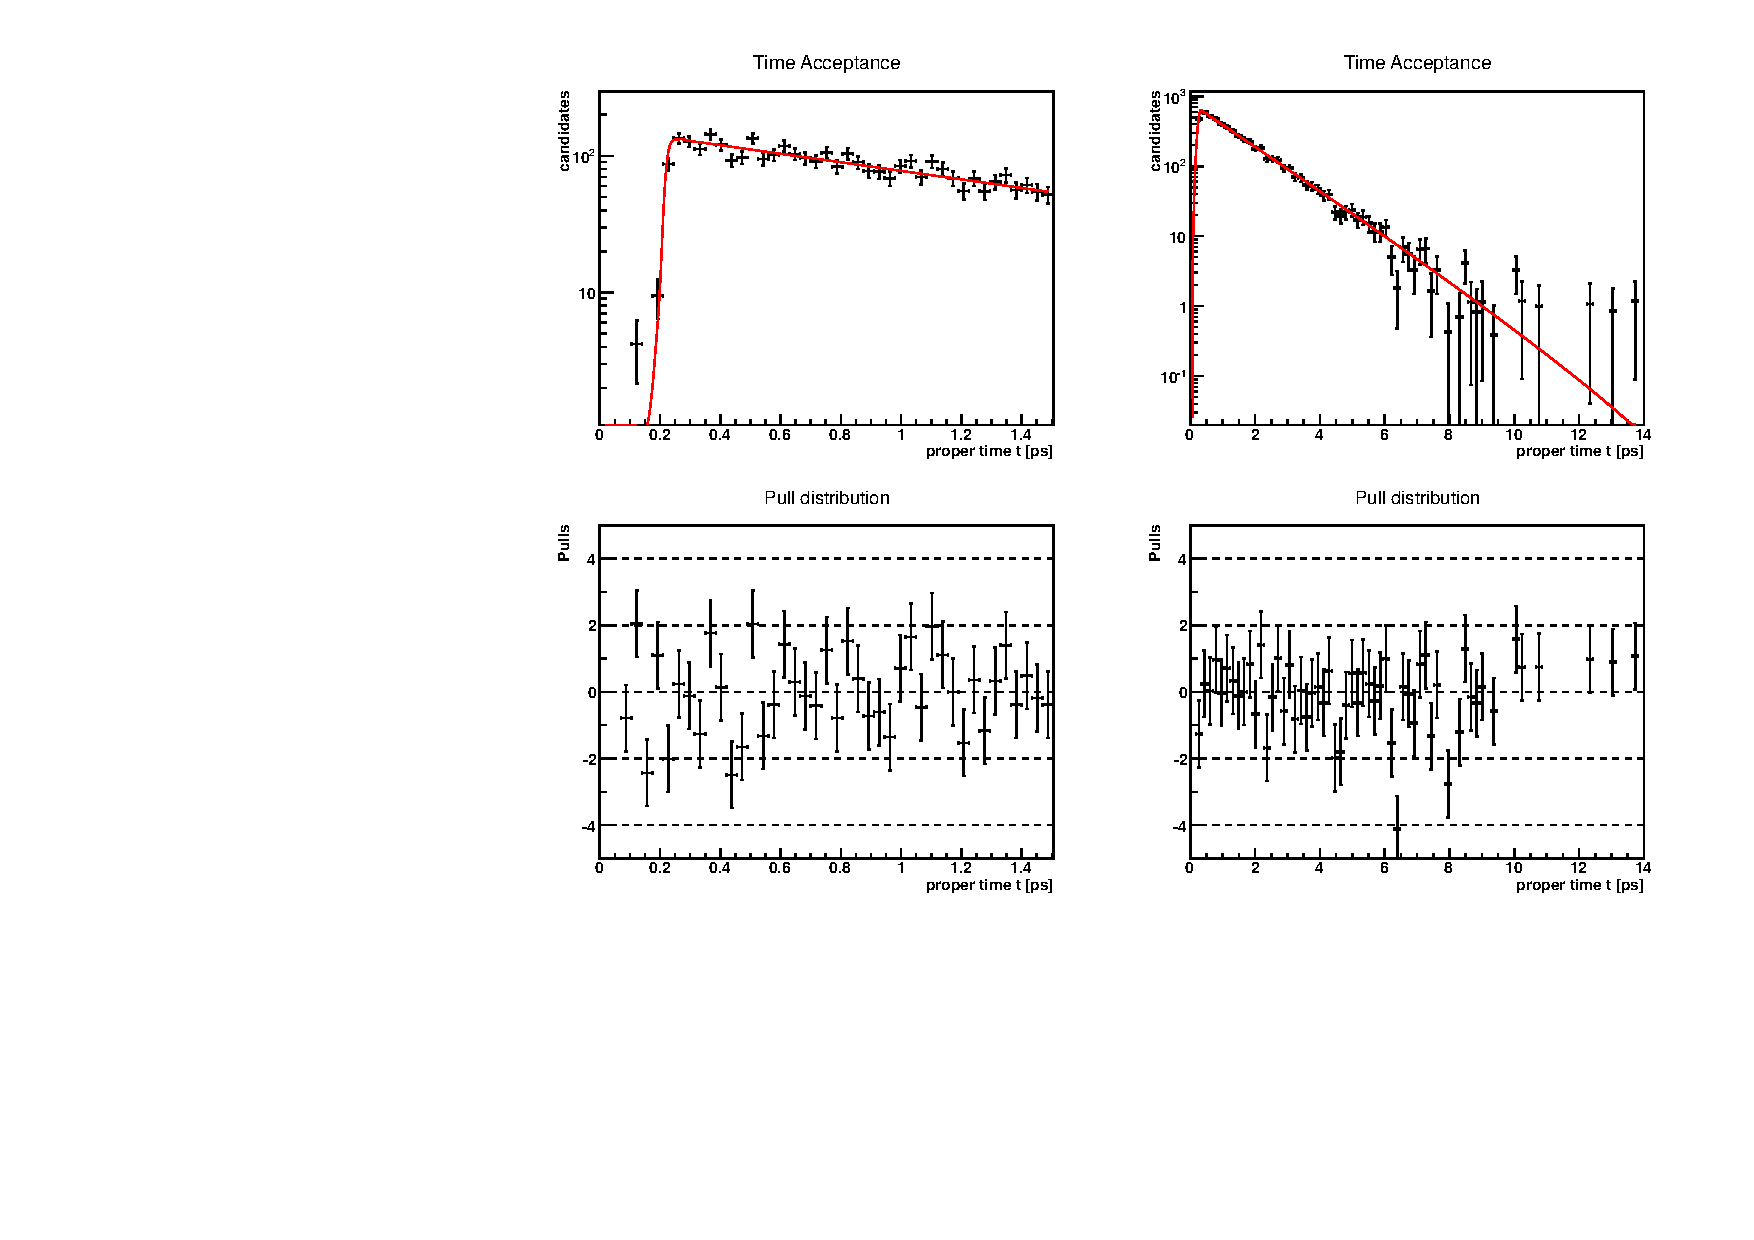
\includegraphics[width=0.85\textwidth]{time_acceptance_fit_lt}
\end{block}
\end{frame}

\begin{frame}{Systematic errors}{Time acceptance}
\begin{block}{Downstream Tracks}
\centering
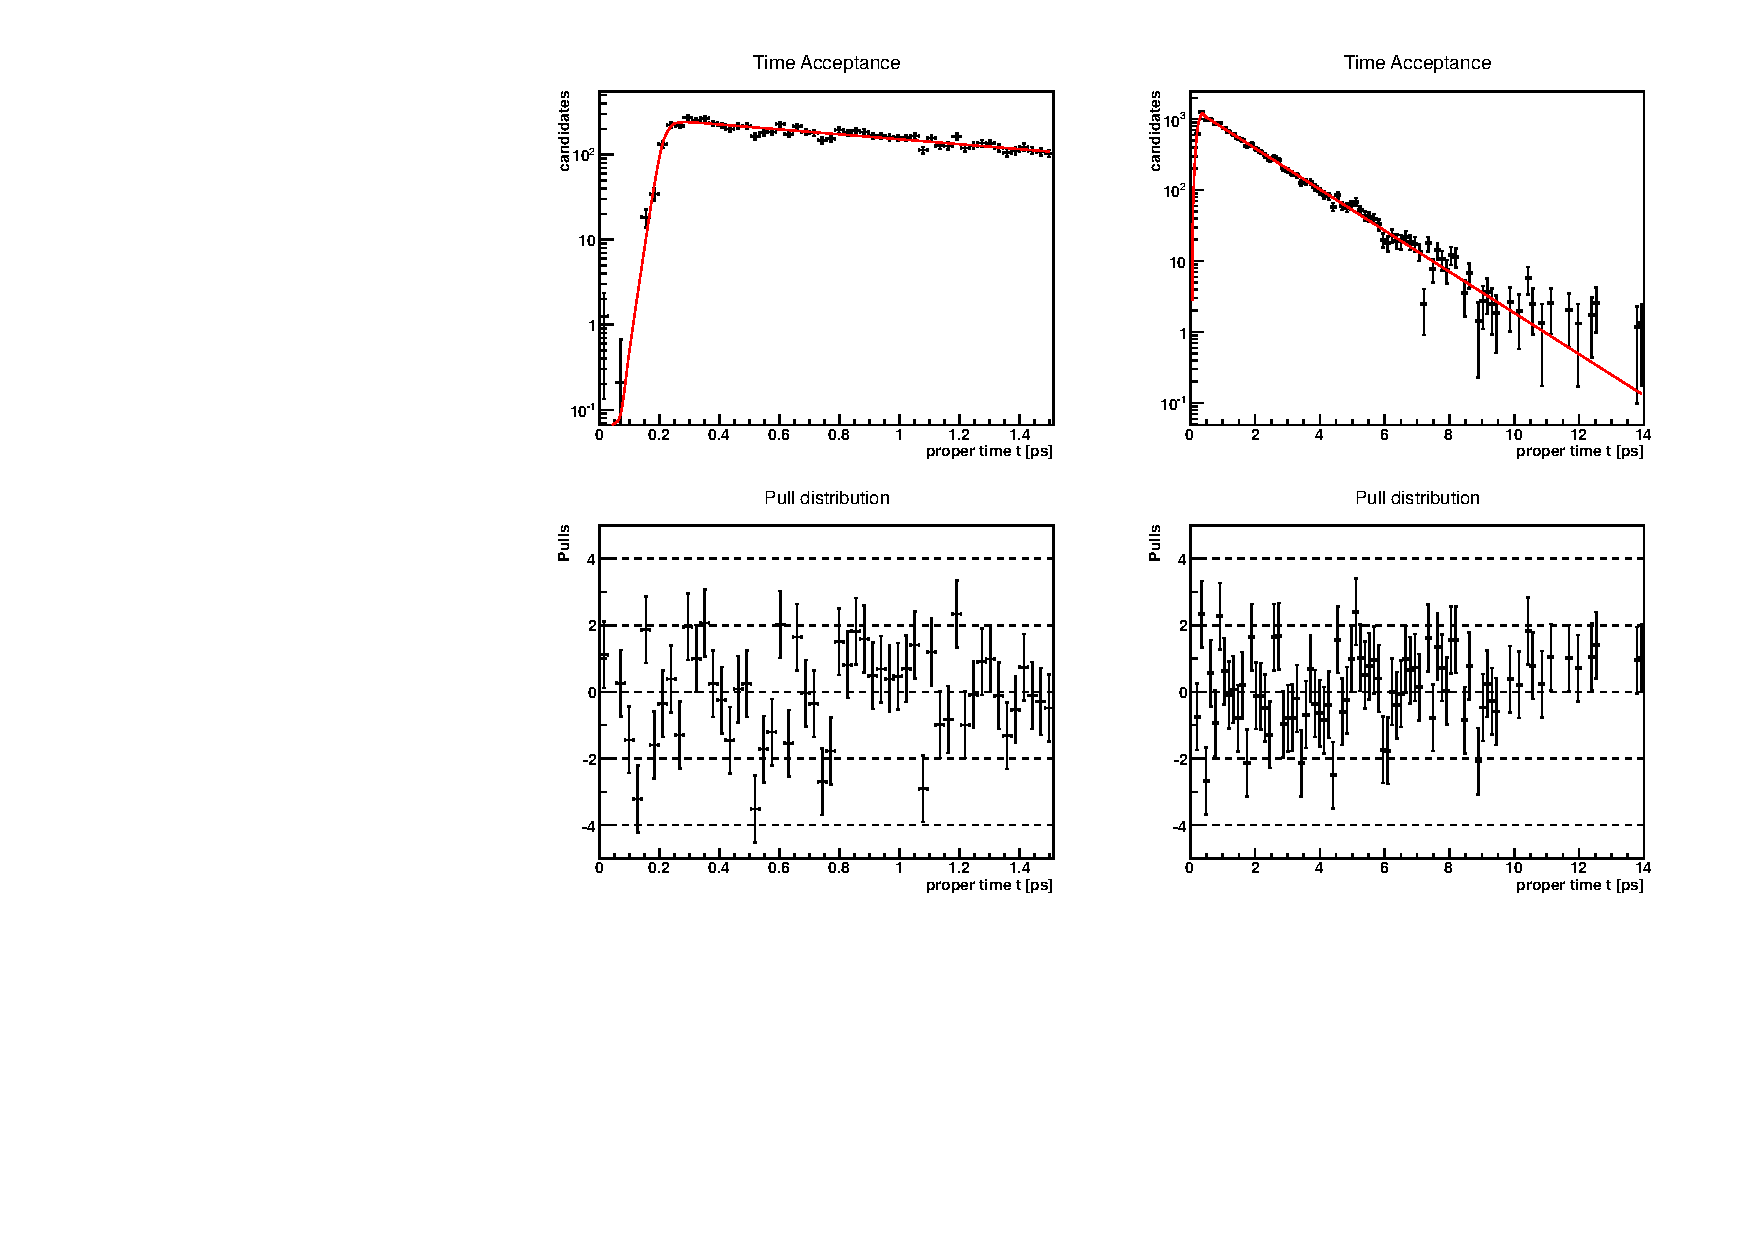
\includegraphics[width=0.85\textwidth]{time_acceptance_fit_ds}
\end{block}
\end{frame}

\begin{frame}{Systematic errors}{Time acceptance}
\begin{table}
\caption{Fit results for exponential decay fit with acceptance function. $\tau$ was constrained to the PDG value $\tau = 1.519 \pm 0.007 \pico\second$}
\begin{tabular}{lr@{$\pm$}l r@{$\pm$}l}
\hline \hline 
parameter & \multicolumn{2}{c}{long} & \multicolumn{2}{c}{downstream} \\ \hline
$\tau$    & 1.518 & 0.007 & 1.519 & 0.007 \\
$a$       & 153 & 36 & 47.9 & 5.6 \\
$b$       & -31.44 & 7.7 & -8.4 & 1.1 \\
$\beta$   & -0.057 & 0.007 &  -0.0090 & 0.0076 \\ 
\hline \hline
\end{tabular}
\end{table}
\end{frame}

\begin{frame}{Systematic errors}{Time acceptance}
Toy MC Study
\begin{itemize}
\item generate with acceptance function 
\item use parameters mentioned above
\item fit without acceptance function
\item compare mean of $\SJPsi$ distribution with corresponding mean of fit bias toy
\end{itemize}

Assignment of systematic error due to neglect of any time acceptance:
	\begin{columns}
	\column{0.5\textwidth}
	\begin{block}{Long Tracks}
    \centering
        $\delta\SJPsi^{\text{Acc}} = 0.0003\ (0.4\%)$
    \end{block}
    	\column{0.5\textwidth}
	\begin{block}{Downstream Tracks}
    \centering
        $\delta\SJPsi^{\text{Acc}} = 0.0008\ (1.3\%)$
    \end{block}
    \end{columns}


\end{frame}

\begin{frame}{Systematic errors}{Correlation mass $\leftrightarrow$ decay time}
Fit reconstructed \Bd-mass in different time bins. Fix mass parameters to the ones obtained in 1 bin and fit $\SJPsi$ in the whole sample.
\begin{center}
\begin{tabular}{c l r@{$\pm$}l r@{$\pm$}l}
\hline \hline
Bin & time range of mass fit & \multicolumn{2}{c}{long} & \multicolumn{2}{c}{down} \\ \hline
1 & $t \in [0.3, 0.7] \pico\second$ & 0.614 & 0.078 & 0.532 & 0.063 \\
2 & $t \in [0.7, 1.5] \pico\second$ & 0.608 & 0.078 & 0.536 & 0.063 \\
3 & $t \in [1.5, 3] \pico\second$ & 0.609 & 0.079 & 0.536 & 0.063 \\
4 & $t \in [3, 14] \pico\second$ & 0.609 & 0.078 & 0.535 & 0.062 \\ \hline
\multicolumn{2}{l}{nominal fit}  & 0.610 & 0.078 & 0.534 & 0.063 \\ \hline
\multicolumn{2}{l}{$\delta\SJPsi^{\text{mass/t}}$} & \multicolumn{2}{c}{0.0020\ (2.6\%)} & \multicolumn{2}{c}{0.0018\ (2.9\%)} \\

\hline \hline
\end{tabular}
\end{center}
\end{frame}

\begin{frame}{Systematic errors}{Resolution}
Vary $\sigma_i$ of resolution $\pm 20\%$, fit with these parameters and compare $\SJPsi$
\begin{center}
\begin{tabular}{c r@{$\pm$}l r@{$\pm$}l}
\hline \hline
 & \multicolumn{2}{c}{long} & \multicolumn{2}{c}{down} \\ \hline
$+20\%$ &0.6100 & 0.0782& 0.5351 & 0.0626 \\
$-20\%$ & 0.6095 & 0.0782 & 0.5345 & 0.0625 \\ \hline
nominal fit & 0.6098 & 0.0782 & 0.5347 & 0.0626 \\ \hline
$\delta\SJPsi^{\text{resolution}}$ & \multicolumn{2}{c}{0.0003\ (0.4\%)} & \multicolumn{2}{c}{0.0004\ (0.6\%)} \\
\hline \hline
\end{tabular}
\end{center}
\end{frame}


\begin{frame}{Systematic errors}{Summary}
\begin{center}
\begin{tabular}{l |c r | c r}
\hline \hline
effect & \multicolumn{2}{c|}{long} & \multicolumn{2}{c}{downstream} \\ \hline
fit  method & 0.0066 & (8.5\%) & 0.0033 & (5.2\%)\\
tagging calibration & 0.0320 & (42.0\%) & 0.0331 & (52.5\%)\\
time acceptance & 0.0003 & (0.4\%) & 0.0008 & (1.3\%)\\
mass $\leftrightarrow$ decay time & 0.0020 & (2.6\%) & 0.0018 & (2.9\%)\\
resolution & 0.0003 & (0.4\%) & 0.0004 & (0.6\%)\\ \hline
total & 0.0328 & (42.1\%) & 0.0333 & (52.9\%)\\ \hline
statistic uncertainty & 0.0782 & & 0.0626 & \\ \hline \hline
\end{tabular}
\end{center}
\end{frame}

\begin{frame}{Conclusion}
	\begin{columns}
	\column{0.5\textwidth}
	\begin{block}{Long Tracks}
	\centering
	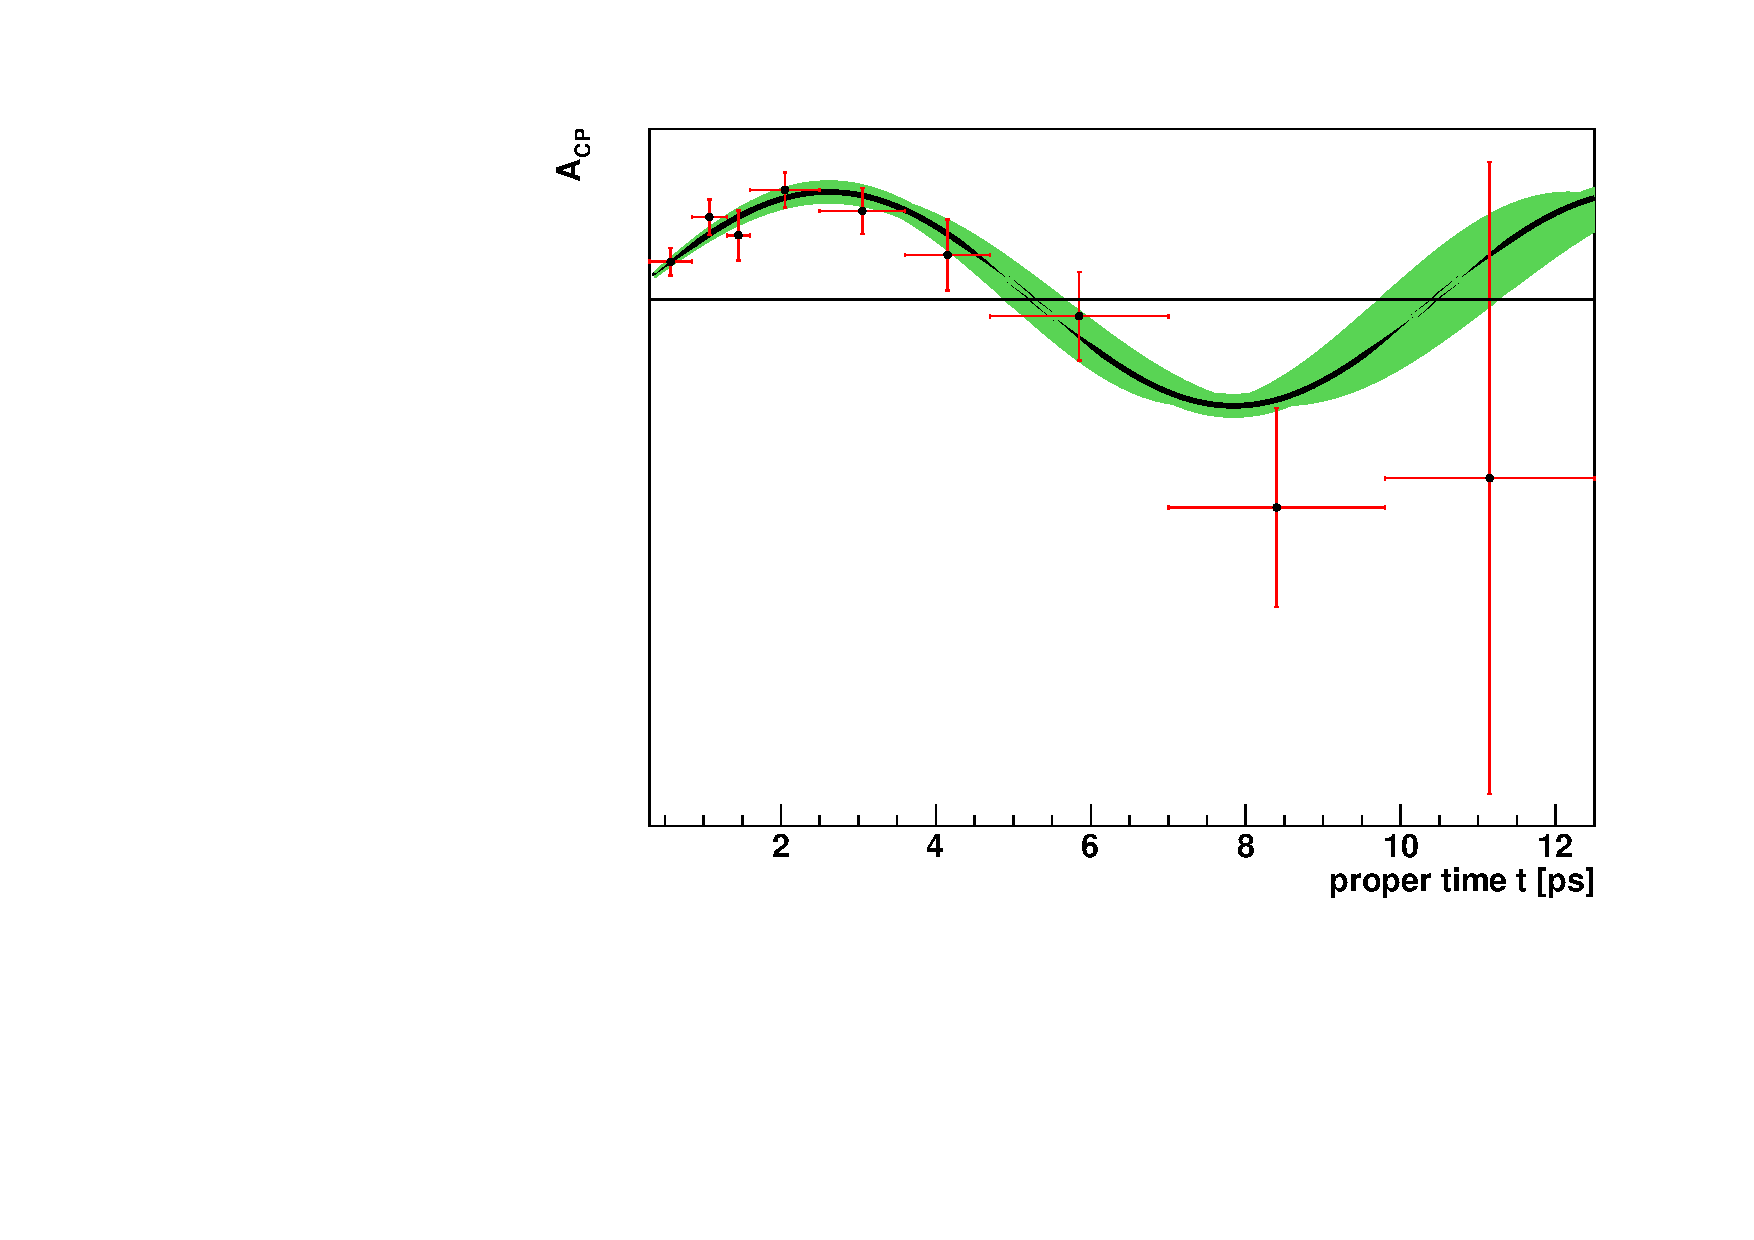
\includegraphics[width=\textwidth]{asymmetry_lt}	
	\end{block}
	$\SJPsi = 0.610 \pm 0.074 (\text{stat.}) \pm 0.033 (\text{syst.})$
	\column{0.5\textwidth}
	\begin{block}{Downstream Tracks}
	\centering
	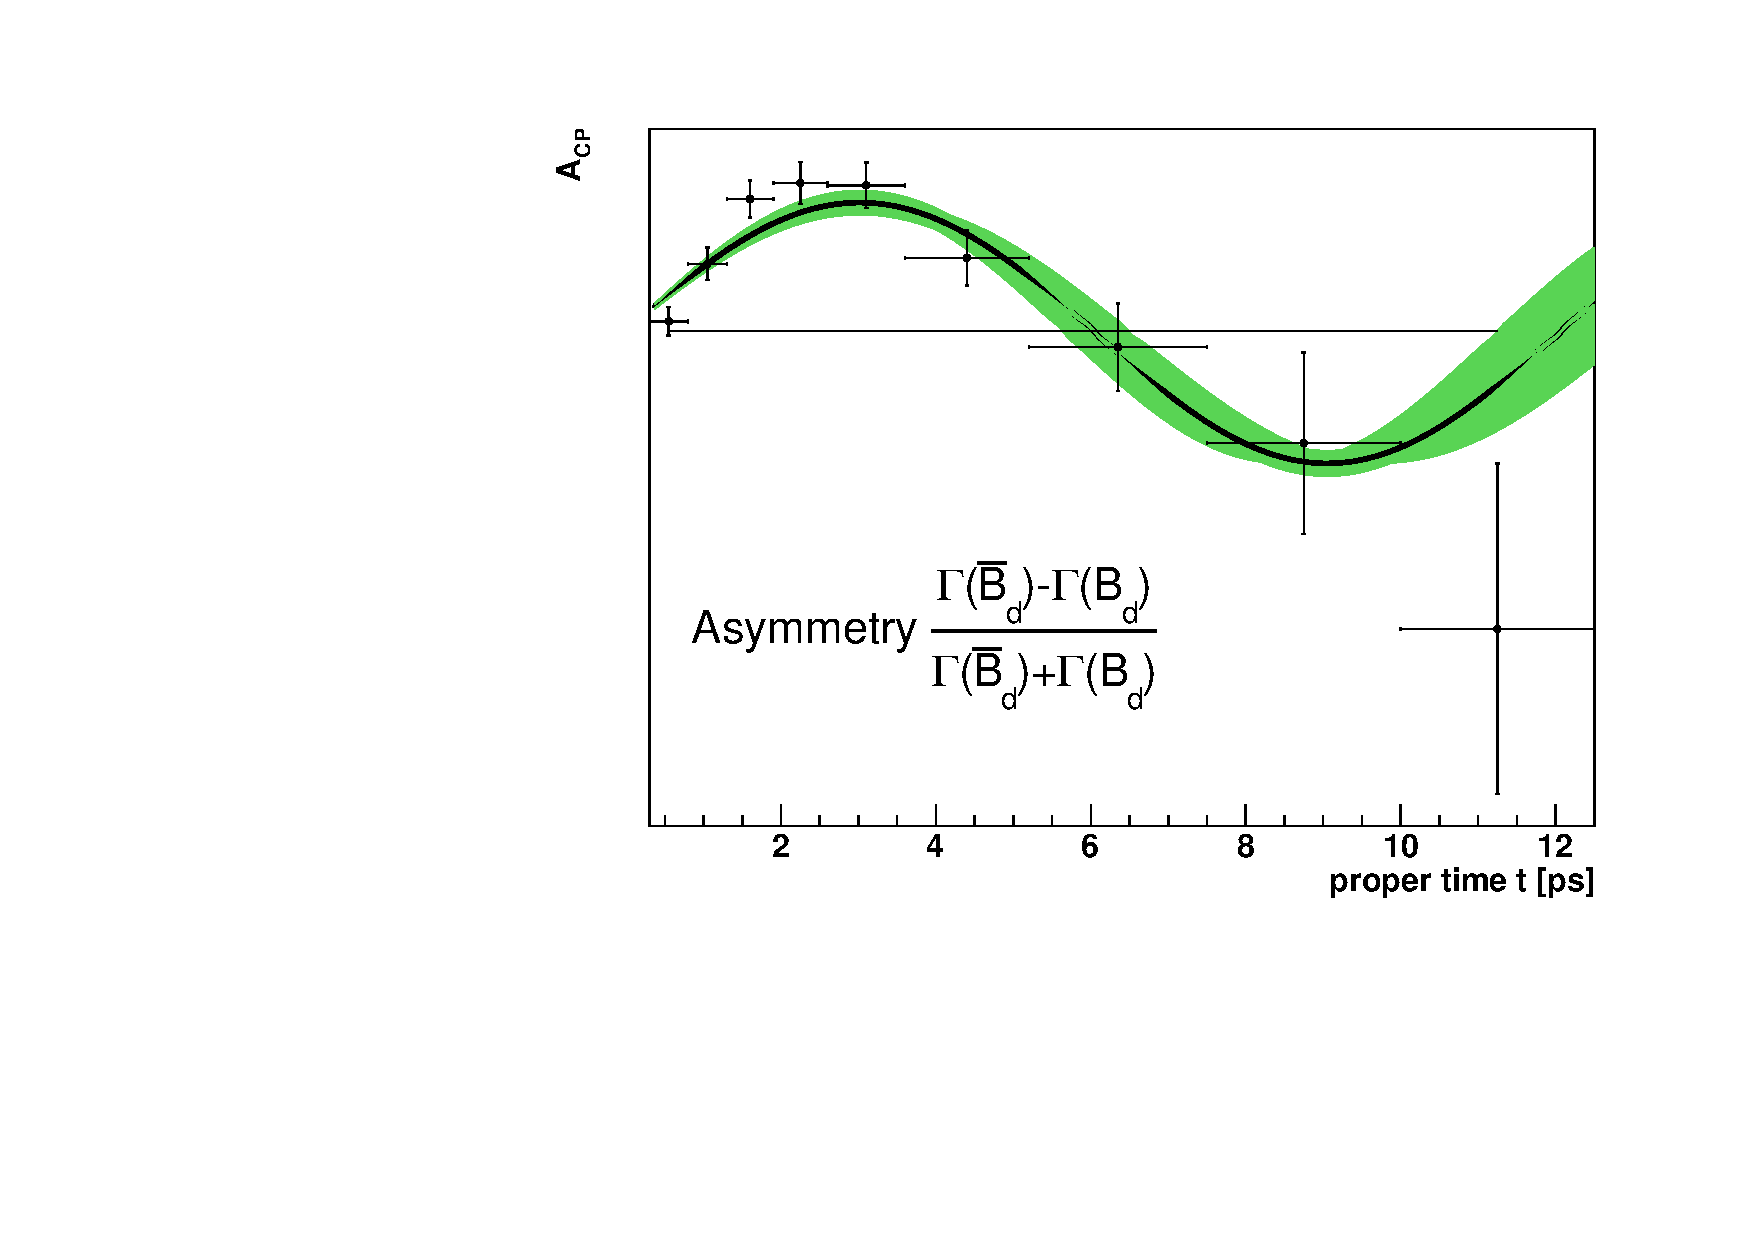
\includegraphics[width=\textwidth]{asymmetry_ds}
	\end{block}
	$\SJPsi = 0.535 \pm 0.059 (\text{stat.}) \pm 0.033 (\text{syst.})$
	\end{columns}
    \begin{center}
    Both results are blinded with the same string. Systematic errors are corrected with $\sigma_{\text{pull}}$ of fit bias toy.
    \end{center}
\end{frame}

\begin{frame}{Conclusion}{Comparison with other results}
\begin{center}
\begin{tabular}{l r@{$\pm$}c@{}l}
\hline \hline
& \multicolumn{3}{c}{$\SJPsi$} \\ \hline
long tracks (blinded) & 0.610 & 0.074 &$\pm$0.033\\
downstream tracks (blinded) & 0.565 & 0.059 &$\pm$0.033\\ \hline
combined & xxx & 0.046&$\pm$0.033 \\ \hline
2011 analysis & 0.72 & 0.06 &$\pm$0.04\\
world average & 0.679 & 0.020 &\\
BaBar (most precise) & 0.687 & 0.028 &$\pm$0.012 \\ \hline \hline
\end{tabular}
\end{center}
\end{frame}

\begin{frame}
\begin{center}
BACKUP
\end{center}
\end{frame}

	
	\begin{frame}{LHCb-detector}
	\begin{center}
	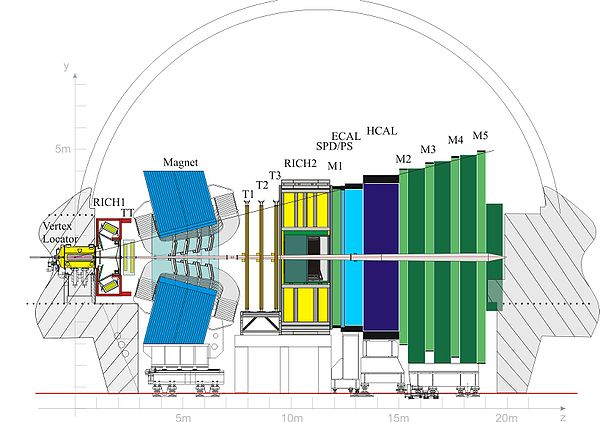
\includegraphics[width = 0.6\textwidth]{detector}
	\end{center}
	\begin{block}{Tracks}
	\begin{itemize}
		\item Long Tracks: VELO + T Stations (Johannes)
		\item Downstream Tracks: TT + T Stations (Patrick)
	\end{itemize}
	\end{block}	
	\end{frame}
	
		\begin{frame}{Decay time fit}{derivation of probability density function}
    \begin{align}
    \mathcal{P}^{true}(\text{\Bd / \Bdbar}) \propto \underbrace{(1\mp             \mu)}_{\text{asymmetric production}} \underbrace{e^{-t/\tau}\left[1\mp \SJPsi \sin(\Delta m_d t)\right]}_{\text{theoretical decay time distribution}}
    \end{align}	
    Imperfect tagging: \\
    \begin{align}
    \mathcal{P}^{meas}(\text{\Bd}) &\propto (1-\omega_{\text{\Bd}})\mathcal{P}^{true}(\text{\Bd}) + \omega_{\text{\Bdbar}} \mathcal{P}^{true}(\text{\Bdbar}) \\
 \mathcal{P}^{meas}(\text{\Bdbar}) &\propto (1-\omega_{\text{\Bdbar}})\mathcal{P}^{true}(\text{\Bdbar}) + \omega_{\text{\Bd}} \mathcal{P}^{true}(\text{\Bd})
    \end{align}

    Combination of all effects and defining 
    \begin{align}
    \Delta p_0 &= \omega_{\text{\Bd}}-\omega_{\text{\Bdbar}} \\
    \omega_{\text{\Bd}/\text{\Bdbar}} &= \omega \pm \frac{\Delta p_0}{2}
    \end{align}
	leads to...
	\end{frame}
	
	\begin{frame}{Decay time fit}{probability density function used in fit}
	\begin{align}
\nonumber\mathcal{P}_{\text{meas}}(t, d, \omega) \propto &e^{-t/\tau} \left\lbrace 1-d\mu(1-2\omega)-d\Delta p_0 \right. \\
&- \left.\left[d(1-2\omega)-\mu(1-d\Delta p_0)\right]\SJPsi\sin(\Delta m_d t)\right\rbrace
	\end{align}
	\begin{itemize}
		\item d: tagging decision
		\item $\mu = A_P = \frac{R_{\bar{B}_d^0}-R_{B_d^0}}{R_{\bar{B}_d^0}+R_{B_d^0}}$ production asymmetry
		\item $\omega$: calibrated mistag probability
		      \begin{align}
		      \omega(\eta^{OS}) = p_1 (\eta^{OS} - \left\langle \eta^{OS} \right\rangle) + p_0
		      \end{align}
		      $p_0, p_1$: calibration parameters \\
		      $\eta^{OS}$: predicted mistag probability
		\item $\Delta p_0$: tagging calibration asymmetry
		\item $\Delta m_d$: mixing frequency

	\end{itemize}	
	\end{frame}
	

% Backup-Folien
% =============
% - Trigger-Definitionen
% - sFit erklären

\end{document}